\documentclass{article}

% Packages
\usepackage[utf8]{inputenc}
\usepackage{subcaption}
\usepackage{enumitem}
\usepackage{titlesec}
\usepackage[T1]{fontenc}
\usepackage[margin=0.7in]{geometry}
\usepackage{subcaption}
\usepackage{graphicx}
\usepackage{array}
\usepackage{amsmath}
\usepackage{amsfonts}
\usepackage{amssymb}
\usepackage{amsthm}
\usepackage{makecell}
\usepackage{gensymb}
\usepackage{multirow}
\usepackage{float}
\usepackage[polish]{babel}
\usepackage{mathptmx}
\usepackage[backend=biber, maxbibnames=3, style=nature, autocite=inline]{biblatex}
\addbibresource{$HOME/Documents/latex/texfiles/bib.bib}

% File-wide formatting and custom commands
\title{Sif}

\renewcommand{\refname}{Na podstawie:}
\renewcommand{\tablename}{\textbf{Tabela}}
\renewcommand{\figurename}{\textbf{Rysunek}}

\setcounter{section}{1}
\setlist{nosep}
\parindent=0in

\newenvironment{nscenter}
 {\parskip=0pt\par\nopagebreak\centering}
 {\par\noindent\ignorespacesafterend}

\newcommand{\punkt}[2]{
\draw [color=black,fill=black] (#1,#2) circle (0.035);}

% Custom table alignments
\newcolumntype{L}[1]{>{\raggedright\let\newline\\\arraybackslash\hspace{0pt}}m{#1}}
\newcolumntype{C}[1]{>{\centering\let\newline\\\arraybackslash\hspace{0pt}}m{#1}}
\newcolumntype{R}[1]{>{\raggedleft\let\newline\\\arraybackslash\hspace{0pt}}m{#1}}

% Custom overline for math mode
\makeatletter
\newsavebox\myboxA
\newsavebox\myboxB
\newlength\mylenA

\newcommand*\xoverline[2][0.75]{%
    \sbox{\myboxA}{$\m@th#2$}%
    \setbox\myboxB\null% Phantom box
    \ht\myboxB=\ht\myboxA%
    \dp\myboxB=\dp\myboxA%
    \wd\myboxB=#1\wd\myboxA% Scale phantom
    \sbox\myboxB{$\m@th\overline{\copy\myboxB}$}%  Overlined phantom
    \setlength\mylenA{\the\wd\myboxA}%   calc width diff
    \addtolength\mylenA{-\the\wd\myboxB}%
    \ifdim\wd\myboxB<\wd\myboxA%
       \rlap{\hskip 0.5\mylenA\usebox\myboxB}{\usebox\myboxA}%
    \else
        \hskip -0.5\mylenA\rlap{\usebox\myboxA}{\hskip 0.5\mylenA\usebox\myboxB}%
    \fi}
\makeatother

% Section Foramtting
\titleformat{\section}
{\sc \bfseries \Large \centering}
{\thesection}
{0,5em}
{}

\titleformat{\subsection}
{\large \bfseries}
{\thesubsection}
{0,5em}
{}

\titleformat{\subsubsection}
{\big \bfseries}
{\thesubsubsection}
{0,5em}
{}

\begin{document}

% Titlepage template by Kacper Nojszewski
\begin{titlepage}
	\begin{center}
	{\scshape\huge Szkoła Główna Gospodarstwa Wiejskiego \par}
	\vspace{0.5cm}
	{\scshape\LARGE Warszawa \par}
	\vspace{0.5cm}
	{\LARGE\bfseries Wydział Ogrodnictwa i Biotechnologii \\ Biotechnologia, rok 3 semestr 5 \par}
	{
\includegraphics[width=0.6\textwidth]{sif.png}}
	\vfill
	%{\input{meta}}

\vfill

% Bottom of the page
	{\LARGE Data \\ <++> \par}
	\end{center}
\end{titlepage}

\tableofcontents

\newpage

\section{Charakterystyka programowo-technologiczna}

Firma kosmetyczna \textsf{Sif} skupia swoją całą uwagę na produkcji kosmetyków do włosów, wyłącznie naturalnych opartych na równowadze PEH i metodzie mycia OMO. Zarówno siedziba firmy kosmetycznej, jak i linia produkcyjna znajdują się w miejscowości Sowia Wola. Jest ona położona w województwie mazowieckim, w powiecie nowodworskim, w gminie Czosnów. Nieduża odległość od miast st. Warszawy (39km), a także bliskie położenie względem Wisłostrady, zapewnia idealny tunel komunikacyjny. Lokalizacja zapewnia możliwość sprawnej dystrybucji produktu. Docelowa produkcja zakładu będzie wynosiła 1\,110 ton kosmetyków.
Produkty dedykowane są osobom, które stosują świadomą pielęgnację włosów lub chcą ją dopiero zacząć. \vspace{\baselineskip}

W dotychczas stworzonej ofercie figurują produkty takie jak.:

\begin{itemize}
	\item 3 Odżywki do włosów:
	\begin{itemize}
	\item Proteinowa;
	\item Emolientowa;
	\item Humektantowa.
	\end{itemize}
	\item 2 Szampony myjące do włosów
	\begin{itemize}
	\item Lekki szampon ziołowy;
	\item Szampon wzbogacony o mocniejszy detergent oraz składniki o właściwościach peelingujących.
	\end{itemize}
\end{itemize}\vspace{\baselineskip}

\textbf{Opisy produktów:}
\begin{itemize}
	\item Odżywka proteinowa -- planowana roczna produkcja wynosi 150 ton (lub 500 tys. butelek o pojemności 300ml). Lekka formuła zbudowana na bazie mleka owsianego i dodatkiem startej kory dębu Nadaje przyjemny zapach. Odżywka wypełnia mikrouszkodzenia, nadaje włosom naturalną objętość i blask.
	\item Odżywka emolientowa -- planowana produkcja roczna wynosi 150 ton (lub 500 tys. butelek o pojemności 300ml). Odżywka do włosów o gęstej formule stworzona z oleju arganowego i oleju z czarnuszki, tworzy zwartą powłokę zabezpieczającą strukturę włosa przez czynnikami mechanicznymi, a dzięki kremowej formule, włosy stają się gładkie i miękkie.
	\item Odżywka humektantowa -- planowna roczna produkcja w wynosi 150 ton (lub 500 tys. butelek o pojemności 300ml). Połączenie olejków z awokado i aloesu, zapewnia właściwe nawilżenie i tym samym zdrowy wygląd włosów.
	\item Lekki szampon ziołowy -- roczna produkcja planowana na 330 ton (lub 660 tys. butelek o pojemności 500ml). Pozbawiony mocnych detergentów, składowo uzupełniony o zioła takie jak liście maliny właściwej, pokrzywy zwyczajnej i tymianku.
	\item Szampon wzbogacony -- planowana roczna produkcja wynosi 330 ton (lub 660 tys. butelek o pojemności 500ml) Zawiera mocniejszy detergent oraz składniki o właściwościach peelingujących, w tym elementy peelingu ze zmielonych ziaren kawy.
\end{itemize}\vspace{\baselineskip}

\textbf{Wszystkie kosmetyki wyróżniają się:}
\begin{itemize}
\item wyłącznie naturalnymi składnikami;
\item składem opartym na równowadze PEH (proteinowo-emolientowo-humektantowej);
\item tym, że są przyjazne dla środowiska (zarówno pod względem składników kosmetyków, jak i opakowań z plastiku biodegradowalnego, we współpracy z zewnętrzną polską firmą ekologiczną);
\item certyfikatem i potwierdzeniem „cruelty free” tj. nietestowaniem produktów na zwierzętach na żadnym etapie produkcji i po jej zakończeniu;
\item wegańskimi składnikami wykluczającymi składniki takie jak: tłuszcze czy białka pochodzenia zwierzęcego.
\end{itemize}\vspace{\baselineskip}

Do produkcji produktów zawierających w sobie zioła używane są ekstrakty ziołowe pochodzenia naturalnego. Ekstrakt z liści maliny używany jest w ilości 26,4 tony w skali roku, a ekstrakt z pokrzywy właściwej w ilości 23,1 tony w skali roku. Ekstrakt z tymianku używany jest w ilości 10,89 tony w skali roku.

Szampon zawierający kawę, zawiera ją w postaci drobno zmielonych ziaren, które używane są w ilości 49,17 tony w skali roku.\vspace{\baselineskip}

Używana w zakładzie woda spełnia standardy sanitarne, a na etapach produkcji najbardziej wrażliwych i narzucających konieczność wysokiej sterylności używana jest woda oczyszczana w systemie Mili-Q.


\section{Baza surowcowa -- charakterystyka surowców (odmiana, jakość surowców, formy oceny jakości)}

\subsection{Składy poszczególnych produktów}

\begin{itemize}
\item odżywka proteinowa
\item odżywka emolientowa
\item odżywka humektantowa
\item szampon ziołowy
\item szampon peelingujący
\end{itemize}\vspace{\baselineskip}

{\renewcommand{\figurename}{\textbf{Tabela}}
\begin{figure}[H]
\centering
	\caption{(a) i (b) składy poszczególnych szamponów. (c), (d) i (e) składy poszczególnych odżywek}
\begin{footnotesize}
	\begin{subfigure}[t]{0.45\textwidth}
		\centering
		\caption{Szampon ziołowy}
		\begin{tabular}{p{0.6\textwidth}ll}
			\hline
			\multirow{2}{*}{\textbf{Składniki}} & \multicolumn{2}{l}{\textbf{Ilość}} \\
			\cline{2-3}
			& \textbf{Procent} & \textbf{Masa} \\
			\hline\hline
			Aqua (Woda) & 54.50 & 396.5g  \\
			Sodium Coco Sulfate & 10.00 & 50g  \\
			Rubus idaeus L. Leaf Extract & 8.00 & 40g  \\
			Urtica dioica L. Leaf Extract & 7.00 & 35g  \\
			Coco-Glucoside & 5.20 & 26g  \\
			Cocamidopropyl Betaine & 4.00 & 20g  \\
			Thymus vulgaris L Leaf Extract & 3.30 & 16.5g  \\
			Sodium Benzoate & 2.50 & 12.5g  \\
			Guar Hydroxypropyltrimonium Chloride & 2.00 & 10g  \\
			Citric Acid & 1.80 & 9g  \\
			Sodium Chloride & 1.50 & 5g  \\
			Tocopherol & 0.20 & 1g  \\
			\hline
		\end{tabular}
	\end{subfigure}
	\begin{subfigure}[t]{0.5\textwidth}
		\centering
		\caption{Szampon peelingujący}
		\begin{tabular}{p{0.6\textwidth}lll}
			\hline
			\multirow{2}{*}{\textbf{Składniki}} & \multicolumn{2}{l}{\textbf{Ilość}} \\
			\cline{2-3}
			& \textbf{Procent} & \textbf{Masa}  \\
			\hline\hline
			Aqua (Woda) & 48.00 & 240g  \\
			Coffea arabica L. Bean Grind & 14.90 & 74.5g  \\
			Sodium Coco Sulfate & 13.50 & 67.5g  \\
			Glycerin & 5.00 & 25g  \\
			Prunus Amygdalus Dulcis (Sweet Almond) Oil & 4.00 & 20g  \\
			Cocamidopropyl Betaine & 4.00 & 20g  \\
			Coco-Glucoside & 4.00 & 20g  \\
			Citric Acid & 2.50 & 17.5g  \\
			Guar Hydroxypropyltrimonium Chloride & 1.90 & 9.5g  \\
			Sodium Benzoate & 1.10 & 5.5g  \\
			Sodium Chloride & 1.00 & 5g \\
			Tocopherol & 0.10 & 0.5g  \\
			\hline
		\end{tabular}
	\end{subfigure}

	\begin{subfigure}[t]{0.45\textwidth}
		\centering
		\caption{Odżywka proteinowa}
		\begin{tabular}{p{0.6\textwidth}lll}
			\hline
			\multirow{2}{*}{\textbf{Składniki}} & \multicolumn{2}{l}{\textbf{Ilość}} \\
			\cline{2-3}
			& \textbf{Procent} & \textbf{Masa} \\
			\hline\hline
			Aqua (Woda)  & 49.00 & 147g \\
			Cetearyl Alkohol  & 22.00 & 66g \\
			Quercus robur L. Bark Extract   & 7.00 & 21g \\
			Glycerin  & 5.00 & 15g \\
			Wheat Amino Acids   & 4.50 & 13.5g \\
			Behentrimonium Chloride  & 4.00 & 12g \\
			Polyglyceryl-3 PCA  & 2.00 & 6g \\
			Potassium Sorbate  & 2.00 & 6g \\
			Sodium Benzoate  & 2.00 & 6g \\
			Dehydroacetic Acid  & 1.00 & 3g \\
			Citric Acid  & 0.90 & 2.7g \\
			Lactic Acid  & 0.20 & 0.6g \\
			Linalool & 0.20 & 0.6g \\
			Tetrasodium EDTA  & 0.20 & 0.6g \\
			\hline
		\end{tabular}
	\end{subfigure}
	\begin{subfigure}[t]{0.5\textwidth}
		\centering
		\caption{Odżywka emolientowa}
		\begin{tabular}{p{0.6\textwidth}ll}
			\hline
			\multirow{2}{*}{\textbf{Składniki}} & \multicolumn{2}{l}{\textbf{Ilość}} \\
			\cline{2-3}
			& \textbf{Procent} & \textbf{Masa} \\
				\hline\hline
				Aqua (Woda) & 40.00 & 120g \\
				Butyrospermum Parkii (Shea Butter) & 14.00 & 42g \\
				Vitis labrusca fruit extract & 9.50 & 28.5g \\
				Argan Oil & 8.50 & 25.5g \\
				Black Cumin Oil & 8.00 & 24g \\
				Cetearyl Alcohol & 7.00 & 21g \\
				Macadamia Ternifolia Seed Oil & 4.00 & 12g \\
				Brassica Oleracea Italica Seed Oil & 3.00 & 9g \\
				Prunus Domestica (Plum) Seed Oil & 3.00 & 9g \\
				Camellia Japonica Seed Oil & 2.00 & 6g \\
				Benzoic Acid & 0.30 & 0.9g \\
				Dehydroacetic Acid & 0.30 & 0.9g \\
				Phenoxyethanol & 0.20 & 0.6g \\
				Linalool & 0.20 & 0.6g \\
			\hline
		\end{tabular}
	\end{subfigure}

	\begin{subfigure}{0.5\textwidth}
		\centering
		\caption{Odżywka humektantowa}
		\begin{tabular}{p{0.6\textwidth}ll}
			\hline
			\multirow{2}{*}{\textbf{Składniki}} & \multicolumn{2}{l}{\textbf{Ilość}} \\
			\cline{2-3}
			& \textbf{Procent} & \textbf{Masa} \\
				\hline\hline
				Aqua (Woda) & 46.00 & 138g \\
				Aloe Barbadensis (Aloe Vera) Leaf Juice & 20.00 & 60g \\
				Cetearyl Alcohol & 10.00 & 30g \\
				Glycerin  & 9.00 & 27g \\
				Persea Gratissima Oil & 7.00 & 21g \\
				Behentrimonium Chloride & 5.00 & 15g \\
				Polyglyceryl-3 PCA & 2.00 & 6g \\
				Benzoic Acid & 0.50 & 1.5g \\
				Dehydroacetic Acid & 0.50 & 1.5g \\
				\hline
			\end{tabular}
	\end{subfigure}
\end{footnotesize}
\end{figure}
}

{\renewcommand{\figurename}{\textbf{Tabela}}
\begin{figure}[H]
\centering
\caption{Planowane roczne zużycie surowców do produkcji:}
\begin{footnotesize}
	\begin{subfigure}{0.7\textwidth}
		\centering
		\caption{szamponów}
		\begin{tabular}{p{0.60\textwidth}ll}
			\hline
			\textbf{Składnik} & \makecell[l]{\textbf{Planowane} \\ \textbf{roczne zużycie}} & \textbf{Uwagi} \\
			\hline\hline
			Aqua (Woda) & 420\,090\,kg & \\
			Sodium Coco Sulfate & 77\,550\,kg & \\
			Coco-Glucoside & 60\,720\,kg & \\
			Coffea arabica L. Bean Grind & 49\,170\,kg & \\
			Sodium Benzoate & 43\,680\,kg & \\
			Rubus idaeus L. Leaf Extract & 26\,400\,kg & \\
			Cocamidopropyl Betaine & 26\,400\,kg & \\
			Urtica dioica L. Leaf Extract & 23\,100\,kg & \\
			Citric Acid & 17\,490\,kg & \\
			Glycerin & 16\,500\,kg & \\
			Prunus Amygdalus Dulcis (Sweet Al- mond) Oil & 13\,200\,kg & \\
			Guar Hydroxypropyltrimonium Chlo- ride & 12\,870\,kg & \\
			Thymus vulgaris L Leaf Extract & 10\,890\,kg & \\
			Sodium Chloride & 6\,600\,kg & \\
			Tocopherol & 990\,kg & \\
			\hline
		\end{tabular}
	\end{subfigure}

	\begin{subfigure}{0.7\textwidth}
		\centering
		\caption{odżywek}
		\begin{tabular}{p{0.60\textwidth}ll}
			\hline
			\textbf{Składnik} & \makecell[l]{\textbf{Planowane} \\ \textbf{roczne zużycie}} & \textbf{Uwagi} \\
			\hline\hline
			Aqua (Woda) & 202\,500\,kg & \\
			Cetearyl Alkohol & 58\,500\,kg & \\
			Aloe Barbadensis (Aloe Vera) Leaf Juice & 30\,000\,kg & \\
			Butyrospermum Parkii (Shea Butter) & 21\,000\,kg & \\
			Glycerin & 21\,000\,kg & \\
			Vitis labrusca fruit extract & 14\,250\,kg & \\
			Behentrimonium Chloride & 13\,500\,kg & \\
			Argan oil & 12\,750\,kg & \\
			Black cumin oil & 12\,000\,kg & \\
			Quercus robur L. Bark Extract & 10\,500\,kg & \\
			Persea Gratissima Oil & 10\,500\,kg & \\
			Wheat Amino Acids & 6\,750\,kg & \\
			Macadamia Ternifolia Seed Oil & 6\,000\,kg & \\
			Polyglyceryl-3 PCA & 6\,000\,kg & \\
			Brassica Oleracea Italica Seed Oil & 4\,500\,kg & \\
			Prunus Domestica (Plum) Seed Oil & 4\,500\,kg & \\
			Camellia Japonica Seed Oil & 3\,000\,kg & \\
			Potassium Sorbate & 3\,000\,kg & \\
			Sodium Benzoate & 3\,000\,kg & \\
			Dehydroacetic Acid & 2\,700\,kg & \\
			Citric Acid & 1\,500\,kg & \\
			Benzoic Acid & 1\,200\,kg & \\
			Linalool & 1\,200\,kg & \\
			Lactic Acid & 450\,kg & \\
			Tetrasodium EDTA & 300\,kg & \\
			Phenoxyethanol & 300\,kg & \\
			\hline
		\end{tabular}
	\end{subfigure}
\end{footnotesize}
\end{figure}
}

\subsection{Charakterystyka poszczególnych składników produktów}

\textbf{Składniki szamponów:}

\begin{itemize}
\item \textbf{Sodium Coco Sulfate}

Sodium Coco Sulfate to sól sodowa siarczanu alkoholi tłuszczowych z oleju kokosowego. Jest półsyntetyczną substancją myjącą pochodzenia roślinnego, a konkretnie - anionowym związkiem powierzchniowo-czynnym. W kosmetykach pełni funkcję detergentu bądź emulgatora. Posiada silne właściwości oczyszczające, pianotwórcze (jest odpowiedzialna za wytwarzanie i stabilizację piany) i antystatyczne (pomaga zapobiec np. nadmiernemu elektryzowaniu włosów). SCS otrzymuje się przy pomocy kwasu siarkowego (VI) lub tlenku siarki (VI), które reagują z alkoholami tłuszczowymi, a następnie zostają zobojętnione. Sodium Coco Sulfate posiada mniejsze potencjalnie drażniące właściwości niż szeroko stosowane w kosmetyce detergenty SLS i SLES, wciąż jednak stanowi dość silny środek myjący.

\item \textbf{Coco-Glucoside}

Poliglukozyd kwasów oleju kokosowego. Niejonowa substancja powierzchniowo czynna. Substancja hydrofilowa, bardzo dobrze rozpuszczalna w wodzie. Bezpieczna dla środowiska - biodegradowalna. Stabilna chemicznie. Niewrażliwa na zmiany pH. Substancja bardzo łagodna dla skóry i błon śluzowych. Łagodzi ewentualne działanie drażniące wywołane przez anionowe substancje powierzchniowo czynne. Substancja myjąca - usuwa zanieczyszczenia z powierzchni skóry i włosów. Emulgator O/W, składnik umożliwiający powstanie emulsji. Substancja pianotwórcza, stabilizująca i poprawiająca jakość piany w mieszaninie z anionowymi substancjami powierzchniowo czynnymi. Pełni rolę modyfikatora reologii (czyli poprawia konsystencję) w preparatach myjących, zawierających anionowe substancje powierzchniowo czynne, dzięki tworzeniu tzw. mieszanych miceli. Ponadto pełni rolę solubilizatora, czyli umożliwia wprowadzanie do roztworu wodnego substancji nierozpuszczalnych lub trudno rozpuszczalnych w wodzie, np. kompozycje zapachowe, wyciągi roślinne, substancje tłuszczowe.

\item \textbf{Glycerin}

Gliceryna, alkohol trójwodorotlenowy. Hydrofilowa substancja nawilżająca. Ma zdolność przenikania przez warstwę rogową naskórka, dzięki czemu pełni rolę promotor przenikania - ułatwia w ten sposób transport innych substancji w głąb skóry. Humektant - zapobiega krystalizacji (wysychaniu) masy kosmetycznej przy ujściu butelki, tuby itp. Wspomaga działanie konserwujące poprzez obniżenie aktywności wody, która jest doskonałą pożywką dla drobnoustrojów.

\item \textbf{Cocamidopropyl Betaine}

Kokamidopropylobetaina. Amfoteryczna substancja powierzchniowo czynna. Substancja myjąca - usuwa zanieczyszczenia z powierzchni skóry i włosów. Substancja bardzo łagodna dla skóry i błon śluzowych, łagodzi ewentualne działanie drażniące anionowych substancja powierzchniowo czynnych. Substancja pianotwórcza, stabilizująca i poprawiająca jakość piany w mieszaninie z anionowymi substancjami powierzchniowo czynnymi. Pełni rolę modyfikatora reologii (czyli poprawia konsystencję) w preparatach myjących, zawierających anionowe substancje powierzchniowo czynne, dzięki tworzeniu tzw. mieszanych miceli.

\item \textbf{Polyglyceryl-3 PCA}

Ester kwasu stearynowego i trójpoliglicerolu. Niejonowa substancja powierzchniowo czynna pochodzenia roślinnego lub zwierzęcego, z estrów polimeru gliceryny i tłuszczowego kwasu stearynowego. Nierozpuszczalna w wodzie. Emolient tłusty, tworzy ochronny i natłuszczający film na powierzchni skóry i włosów, który kondycjonuje, zmiękcza i wygładza powierzchnię. Ma również właściwości emulgatora do tworzenia emulsji typu

O/W, zapobiega rozwarstwianiu faz, jest substancją pianotwórczą i myjącą oraz zdolną do tworzenia miceli w produktach z anionowymi surfaktantami. Podwyższa lepkość.

\item \textbf{Prunus Amygdalus Dulcis (Sweet Almond) Oil}

Olej ze słodkich migdałów ma bursztynowy kolor oraz lekki charakterystyczny zapach. W temperaturze pokojowej jest ciekły. Olej ze słodkich migdałów zawiera kwas oleinowy, linolowy oraz witaminy: A, B1, B2, B6, D i E. Tłoczony z nasion drzewa migdałowego. Emolient tzw. tłusty. Jeśli jest stosowany na skórę w stanie czystym, może być komedogenny, czyli sprzyjać powstawaniu zaskórników. Zastosowany w preparatach do pielęgnacji skóry i włosów tworzy na powierzchni warstwę okluzyjną (film), która zapobiega nadmiernemu odparowywaniu wody z powierzchni (jest to pośrednie działanie nawilżające), przez co kondycjonuje, czyli zmiękcza i wygładza skórę i włosy.

%\item \textbf{Glyceryl Oleate}

%Monogliceryd kwasu oleinowego. Niejonowa substancja powierzchniowo czynna. Nierozpuszczalna w wodzie. Stabilna w kwaśnym pH, niestabilna w silnie alkalicznym. Kompatybilna z twardą wodą, zawierającą głównie jony wapnia i magnezu. Emolient tzw. tłusty - stosowany w formie nierozcieńczonej może powodować powstawanie zaskórników. Zastosowany w preparatach do pielęgnacji skóry i włosów tworzy na ich powierzchni warstwę okluzyjną (film), która zapobiega nadmiernemu odparowywaniu wody z powierzchni (jest to pośrednie działanie nawilżające), przez co kondycjonuje skórę i włosy. Powstały film, wygładza powierzchnię naskórka i włosów. Nadaje połysk. Substancja zwilżająca - ułatwia usuwanie zanieczyszczeń. W preparatach myjących stosowany jako substancja renatłuszczająca.Proces mycia powoduje usunięcie m.in. substancji tłuszczowych, dlatego stosuje się substancje renatłuszczające, które odbudowują barierę lipidową. Emulgator W/O, składnik umożliwiający powstanie emulsji.

\item \textbf{Citric Acid}

Kwas cytrynowy należy do grupy alfahydroksykwasów (AHA). Substancja rozpuszczalna w wodzie. Substancja należy do alfahydroksykwasów (AHA) wykazuje działanie keratolityczne, czyli złuszczające, dzięki czemu usuwa przebarwienia i rozjaśnia skórę. Pełni rolę sekwestranta, czyli substancji, która kompeksuje jony metali, dzięki czemu zwiększa trwałość kosmetyku oraz jego stabilność. Regulator pH.

\item \textbf{Guar Hydroxypropyltrimonium Chloride}

Antystatyk tworzący na włosach ochronną powłokę, dodatkowo ma również właściwości odżywcze, wygładza, wzmacnia włosy, ułatwia rozczesywanie.

%\item \textbf{Hydrogenated Palm Glycerides Citrate}

%Utwardzone (Uwodornione) glicerydy palmy olejowej z kwaskiem cytrynowym. Ester kwasku cytrynowego w uwodornionych poprzez przyłączenie atomów wodoru glicerydach/tłuszczach palmy olejowej. Substancja słabo rozpuszczalna w wodzie. Emulgator do tworzenia emulsji typu O/W oraz substancja myjąca. Ma także właściwości kondycjonujące.

\item \textbf{Sodium Chloride}

Nieorganiczny związek chemiczny. Występuje w postaci bezbarwnych kryształów. Dobrze rozpuszcza się w wodzie. Modyfikator reologii. Wpływa na konsystencję kosmetyków myjących - powoduje wzrost lepkość w preparatach zawierających anionowe substancje powierzchniowo czynne.

\item \textbf{Potassium Sorbate}

Sorbinian potasu. Sól kwasu karboksylowego. Występuje w postaci białego, krystalicznego proszku. Substancja konserwująca, która uniemożliwia rozwój i przetrwanie mikroorganizmów w czasie przechowywania produktu. Chroni również kosmetyk przed wtórnym zakażeniem mikroorganizmami które możemy wprowadzić przy codziennym użytkowaniu produktu. Składnik dozwolony do stosowania w kosmetykach w ograniczonym stężeniu. Znajduje się na liście substancji konserwujących dozwolonych do stosowania z ograniczeniami w produktach kosmetycznych. Jego dopuszczalne maksymalne stężenie w gotowym produkcie to 0,6\% w przeliczeniu na kwas sorbowy.

\item \textbf{Sodium Benzoate}

Sól kwasu benzoesowego. Substancja konserwująca, która uniemożliwia rozwój i przetrwanie mikroorganizmów w czasie przechowywania produktu. Chroni również kosmetyk przed nadkażeniem bakteryjnym, które możemy wprowadzić przy codziennym użytkowaniu produktu. Składnik dozwolony do stosowania w kosmetykach w

ograniczonym stężeniu. Znajduje się na liście substancji konserwujących dozwolonych do stosowania z ograniczeniami w produktach kosmetycznych Jego dopuszczalne maksymalne stężenie to 0,5\% (w przypadku stosowania soli tego kwasu jest to 0,5\% w przeliczeniu na czysty kwas benzoesowy).

\item \textbf{Tocopherol}

Witamina E. Organiczny związek chemiczny zawierający w swojej strukturze pierścień 6-chromanolu, do którego dołączony jest izoprenowy łańcuch boczny. Nierozpuszczalny w wodzie. Rozpuszczalny w węglowodorach, alkoholach, tłuszczach i olejach. Określenie "witamina E" odnosi się do grupy związków naturalnych, w skład której wchodzą tokoferole i tokotrienole. Najwyższą aktywność biologiczą wykazuje D-$\alpha$-tokoferol, który jest głównym składnikiem naturalnej witaminy E. Substancja o działaniu antyoksydacyjnym (przeciwutleniającym), hamuje procesy starzenia się skóry wywoływane np. promieniowaniem UV lub dymem papierosowym. Jest doskonałym czynnikiem hamującym rodnikowe utlenianie lipidów w naskórku i skórze właściwej. Witamina E wykazuje zdolność wbudowywania się w struktury lipidowe błon komórkowych i cementu międzykomórkowego warstwy rogowej, dzięki czemu wzmacnia barierę naskórkową. Wzmocnienie bariery naskórkowej nie tylko utrudnia wnikanie substancji obcych i zapobiega podrażnieniom, ale także hamuje TEWL (transepidermalną utratę wody) dzięki czemu wpływa na poprawę nawilżenia skóry. Zapobiega powstawaniu stanów zapalnych, wzmacnia ściany naczyń krwionośnych i poprawia ukrwienie skóry. Przeciwutleniacz (antyoksydant). Zapobiega lub w znaczny sposób ogranicza szybkość zachodzenia procesu utleniania zawartych w kosmetyku składników tłuszczowych, np. niektórych cennych olejów roślinnych. Dodatek antyoksydantów zapewnia trwałość produktów, wydłuża ich przydatność do użycia, zabezpiecza przed powstawaniem nieprzyjemnego zapachu, zmianami barwy oraz konsystencji produktu gotowego.

\item \textbf{Linalool}

Nienasycony alkohol alifatyczny z grupy terpenów. Imituje zapach konwalii. Znajduje się na liście potencjalnych alergenów.

%\item \textbf{Limonene}

%Jednopierścieniowy weglowodór terpenowy. Imituje zapach skórki cytrynowej. Znajduje się na liście potencjalnych alergenów.

%\item \textbf{Geraniol}

%Nienasycony alkohol alifatyczny z grupy terpenów. Imituje zapach pelargonii. Znajduje się na liście potencjalnych alergenów.
\end{itemize}

\textbf{Składniki odżywek:}

\begin{itemize}
\item \textbf{Macadamia Ternifolia Seed Oil}

Olej z nasion makadamia. Jasnożółty olej otrzymywany poprzez tłoczenie nasion makadamii. Zawiera 57\% kwasu olejowego, 25\% kwasu palmitynowego, 15\% nasyconych kwasów tłuszczowych, bogaty w witaminy: A, B, E oraz składniki mineralne. Emolient tzw. tłusty. Jeśli jest stosowany na skórę w stanie czystym, może być komedogenny, czyli sprzyjać powstawaniu zaskórników. Zastosowany w preparatach do pielęgnacji skóry i włosów tworzy na ich powierzchni warstwę okluzyjną (film), która zapobiega nadmiernemu odparowywaniu wody z powierzchni (jest to pośrednie działanie nawilżające), przez co kondycjonuje skórę i włosy. Powstały film, wygładza powierzchnię naskórka i włosów.

\item \textbf{Cetearyl Alcohol}

Mieszanina alkoholu cetylowego i stearylowego. Niejonowa substancja powierzchniowo czynna. Alkohol cetylowy i alkohol stearylowy są głównymi składnikami tworzącymi alkohol cetylostearylowy. Należy do alkoholi tłuszczowych. Ma konsystencję stałego wosku. Emolient tzw. tłusty. Jeśli jest stosowany na skórę w stanie czystym, może być komedogenny, czyli sprzyjać powstawaniu zaskórników. Zastosowany w preparatach do pielęgnacji skóry i włosów tworzy na powierzchni warstwę okluzyjną (film), która zapobiega nadmiernemu odparowywaniu wody z powierzchni (jest to pośrednie działanie nawilżające), przez co kondycjonuje, czyli zmiękcza i wygładza skórę i włosy. Substancja konsystencjotwórcza, wpływa na lepkość gotowego produktu i poprawia właściwości użytkowe (aplikacyjne). Stabilizator emulsji.

\item \textbf{Behentrimonium Chloride}

Chlorek dokozylotrójmetyloamoniowy.. Czwartorzędowa sól amoniowa. Substancja łatwopalna, żółta, woskopodobna, pochodna tłuszczowego alkoholu behenowego pochodzenia roślinnego lub z wosku pszczelego. Rozpuszczalna w gorącej wodzie lub tłuszczach. Dopuszczalne stężenie w kosmetykach 0,1\%. Substancja bardzo często stosowana w produktach do mycia oraz pielęgnacji włosów, szamponach, odżywkach, maskach. Ma działanie myjące, zapobiega elektryzowaniu i plątaniu włosów, ułatwia rozczesywanie, wygładza, zmiękcza i kondycjonuje. Wykazuje również lekkie działanie konserwujące.

\item \textbf{Brassica Oleracea Italica Seed Oil}

Olejek pozyskiwany z nasion brokułu. Szczególnie nadaje się do pielęgnacji włosów, nadaje włosom połysk, może być użyty jako zastępstwo silikonów. On ma silne działanie kondycjonowania i wygładzania, łagodzi skręcanie się włosów.

\item \textbf{Moringa Oleifera Seed Oil}

Olej z nasion Moringi Olejodajnej. Olej bogaty w kwas oleinowy. Emolient, tworzy warstwę okluzyjną (film) na powierzchni skóry i włosów, która zapobiega nadmiernemu odparowywaniu wody z powierzchni (pośrednie działanie nawilżające). Działa kondycjonująco, nawilżająco i regenerująco.

\item \textbf{Prunus Domestica (Plum) Seed Oil}

Olej z pestek śliwki/olej śliwkowy. Ma działanie antyoksydacyjne i przeciwzapalne. Zawiera kwas oleinowy (do 80\%), nie pozostawia lepkiej warstwy i bardzo szybko się wchłania. Idealnie nadaje się do masażu ciała i twarzy. Działa kojąco i nawilżająco, a zawarte w nim fitosterole wpływają na poprawę jędrności skóry, wykazując działanie przeciwzmarszczkowe. Jako dodatek w mieszankach olejowych przedłuża trwałość delikatnych, podatnych na psucie olejów, zmniejsza wrażenie tłustości, przyspiesza wchłanianie oraz wzmacnia przenikanie składników aktywnych do głębszych warstw skóry. Olej śliwkowy jest również bogaty w witaminę E, która pełni funkcję antyoksydantu, zwalczającego wolne rodniki, dzięki temu olej chroni strukturę skóry przed zniszczeniami powodowanymi czynnikami zewnętrznymi.

\item \textbf{Camellia Japonica Seed Oil}

Olejek Tsubaki. Uzyskany z cennej odmiany kamelii, posiada niezwykłe właściwości odżywcze, zmiękczające i regenerujące, zapobiega przedwczesnemu starzeniu się włosów; nadaje matowym włosom połysk i witalność oraz sprawia, że stają się mocniejsze i grubsze.

%\item \textbf{Starch Hydroxypropyltrimonium Chloride}

%Emolinet, regulator lepkości, substancja antysatyczna. W szamponach i odżywkach do włosów, sprawia, że włosy są łatwe do rozczesania, elastyczne, miękkie i lśniące.

%\item \textbf{Cetrimonium Chloride}

%Chlorek cetylotrójmetyloamoniowy Nazwa zwyczajowa: Czwartrzędowa sól amoniowa. Kationowa substancja powierzchniowo czynna. Dzięki temu, że substancja posiada ładunek dodatni z łatwością łączy się z ujemnie naładowaną powierzchnią włosa. Substancja kondycjonująca włosy: poprawia rozczesywalność, zapobiega splątywaniu, nadaje połysk i wygładza włosy, wykazuje działanie antystatyczne, dzięki czemu zapobiega elektryzowaniu się włosów. Ułatwia spłukiwanie preparatu. Cetrimonium Chloride również obniża napięcie międzyfazowe, co ułatwia łączenie się fazy wodnej i olejowej. Substancja konserwująca, która uniemożliwia rozwój i przetrwanie mikroorganizmów w czasie przechowywania produktu. Chroni również kosmetyk przed nadkażeniem bakteryjnym, które możemy wprowadzić przy codziennym użytkowaniu produktu. Składnik dozwolony do stosowania w kosmetykach w ograniczonym stężeniu. Znajduje się na liście substancji konserwujących dozwolonych do stosowania z ograniczeniami w produktach kosmetycznych. Jego dopuszczalne maksymalne stężenie w gotowym produkcie wynosi 0,1\% (jeżeli składnik pełni rolę substancji konserwującej).

\item \textbf{Phenoxyethanol}

Fenoksyetanol. Substancja konserwująca, która uniemożliwia rozwój i przetrwanie mikroorganizmów w czasie przechowywania produktu. Chroni również kosmetyk przed zakażeniem bakteryjnym, które możemy wprowadzić przy codziennym użytkowaniu produktu. Składnik dozwolony do stosowania w kosmetykach w ograniczonym stężeniu. Znajduje się na liście substancji konserwujących dozwolonych do stosowania z ograniczeniami w produktach kosmetycznych. Jego dopuszczalne maksymalne stężenie w gotowym produkcie to 1,0\%

\item \textbf{Benzoic Acid}

Kwas benzoesowy. Substancja konserwująca, która uniemożliwia rozwój i przetrwanie mikroorganizmów w czasie przechowywania produktu. Chroni również kosmetyk przed nadkażeniem bakteryjnym, które możemy wprowadzić przy codziennym użytkowaniu produktu. Kwas benzoesowy jest dozwolony do stosowania w kosmetykach w ograniczonej ilości. Znajduje się na liście substancji konserwujących dozwolonych do stosowania. Ze względu na szerokie zastosowanie tego związku w różnego rodzaju preparatach dopuszczalne jest różne jego stężęnie w zależności od rodzaju kosmetyku. Maksymalne stężenie kwasu benzoesowego i jego soli sodowej w gotowym kosmetyku wynosi:

produkty spłukiwane z wyjątkiem preparatów do jamy ustnej: do 2,5\% (w przeliczeniu na czysty kwas benzoesowy, w przypadku stosowania soli sodowej kwasu benzoesowego);

produkty do jamy ustnej: do 1,7\% (w przeliczeniu na czysty kwas benzoesowy, w przypadku stosowania soli sodowej kwasu benzoesowego);

produkty niespłukiwane: do 0,5\% (w przeliczeniu na czysty kwas benzoesowy, w przypadku stosowania soli sodowej kwasu benzoesowego);

inne pochodne we wszystkich wyrobach do 0,5\% (w przeliczniu na czysty kwas benzoesowy).

\item \textbf{Dehydroacetic Acid}

Kwas dehydrooctowy. Substancja otrzymywana naturalnie lub syntetycznie, lecz identyczna z występującym w naturze kwasem dehydrooctowym. Dopuszczalne stężenie w kosmetykach: 0,6\%. Łagodny konserwant. Zapobiega zepsuciu kosmetyku, chroni przed mikroorganizmami.
\end{itemize}


\nocite{Grote1988, Oh1987, Leite2020, Ziaja, 4Szpaki, Kosmopedia, KosmetykWszechCzasów, SubiektynikKosmetyczny, Loczek}

\section{Organizacja skupu i transportu. Warunki skupu i dostaw surowca}

\subsection{Woda destylowana}
%
%\textbf{Przykładowe obliczenia:}
%
%Zawartość wody w 1 butelce szamponu ziołowego wynosi 396,5g a w 1 butelce szamponu peelingującego - 240g, co przy rocznej produkcji w ilości 660 tys. każdego szamponu daje roczne zapotrzebowanie na wodę równe 420090l (((396.5+240)*660tys)/1000). Tygodniowe zapotrzebowanie na wodę wynosi więc 8752l (420090/(12*4)). Liczba zamawianych paletopojemników wynosi zatem 9 (8752/1000). \vspace{\baselineskip}
%
%Obliczenia w przypadku pozostałych substancji zostały wykonane analogicznie.
%
%Woda będzie dostarczana do nas przez firmę zewnętrzną Czysta Woda Śląsk w paletopojemnikach o pojemności 1000l w ilości 9 sztuk raz w tygodniu, w każdą środę o godz. 7.00. Paletopojemniki będziemy od nich dzierżawili i odsyłali po kolejnym zamówieniu. \vspace{\baselineskip}
%
%O wyborze dostawcy zadecydowała korzystna oferta przedstawiona przez firmę dotycząca cen oraz dostaw, a także wysokie standardy jakościowe produktu.
%
%\subsection{Sodium Coco Sulfate}
%
%Będzie dostarczany przez firmę OQEMA w workach o pojemności 50 kg w ilości 130 sztuk raz w miesiącu.
%
%\subsection{Coco-Glucoside}
%
%Glukozyd kokosowy będzie dostarczany przez firmę OQEMA w beczkach o pojemności 220 kg w ilości 12 sztuk raz w miesiącu. Beczki będą dzierżawione i odsyłane po kolejnym zamówieniu.
%
%\subsection{Glycerin}
%
%Gliceryna będzie dostarczana przez firmę OQEMA w paletopojemnikach o pojemności 500 kg w ilości 3 sztuk raz w miesiącu. Paletopojemniki będziemy od nich dzierżawili i odsyłali po kolejnej dostawie.
%
%\subsection{Prunus Amygdalus Dulcis (Sweet Almond) Oil}
%
%Olej migdałowy będzie dostarczany przez firmę OQEMA w beczkach o pojemności 600kg w ilości 2 sztuk raz w miesiącu. Beczki będą dzierżawione i odsyłane po kolejnym zamówieniu. 
%
%\subsection{Tocopherol}
%
%Będzie dostarczany w postaci octanu tokoferylu przez firmę OQEMA w opakowaniach 25kg w ilości 4 sztuk raz w miesiącu. 
%
%Zgodnie z umową, firma OQEMA będzie odpowiedzialna za dostawy powyższych produktów, które będą odbywały się w każdą pierwszą środę miesiąca o godz. 8.00.
%O wyborze tego dostawcy zadecydowała bliskość magazynu firmy OQEMA, wysoka jakość oferowanych produktów, a także gotowość producenta do przygotowania mieszanek na specjalne życzenie klienta.
%
%\subsection{Coffea arabica L. Bean Grind}
%Kawa arabska będzie dostarczana przez firmę TRB Natural Extract w bębnach z włókniny o pojemności 25 kg w ilości 170 sztuk raz w miesiącu.
%
%\subsection{Urtica dioica L. Leaf Extract}
%
%Ekstrakt z pokrzywy zwyczajnej będzie dostarczany przez firmę TRB Natural Extract w bębnach z włókniny o pojemności 25 kg w ilości 77 sztuk raz w miesiącu. 
%
%Zgodnie z umową zawartą z firmą TRB Natural Extract będzie ona zajmowała się dostawami zamawianych produktów, które będą realizowane w każdą pierwszą środę miesiąca o godz. 9.00.
%
%O wyborze dostawcy zadecydowało wieloletnie doświadczenie firmy w produkcji naturalnych ekstraktów, udokumentowane wieloma certyfikatami.
%
%\subsection{Cocamidopropyl Betaine}
%
%Kokoamidopropylobetaina będzie dostarczana przez firmę Distripark w beczkach o pojemności 120 kg w ilości 19 sztuk raz w miesiącu.
%
%\subsection{Citric Acid}
%
%Kwas cytrynowy będzie dostarczany przez firmę Distripark w 25 kg workach w ilości 59 sztuk raz w miesiącu.
%
%\subsection{Sodium Benzoate}
%
%Benzoesan sodu będzie dostarczany przez firmę Distripark w workach 25kg w ilości 40 sztuk raz w miesiącu.
%
%Zgodnie z umową zawartą z firmą Distripark, producent jest zobowiązany dostarczać powyższe produkty w każdą pierwszą środę miesiąca o godz. 10.00.
%O wyborze dostawcy zadecydowała wysoka jakość produktów.
%
%\subsection{Sodium Chloride}
%
%Chlorek sodu będzie dostarczany przez firmę CIECH S.A. w workach o pojemności 25kg w ilości 2 sztuk raz w miesiącu oraz w big bagach o pojemności 500kg w ilości 1 sztuki raz w miesiącu. 
%
%Zgodnie z umową, za dostawę chlorku sodu odpowiedzialny będzie producent. Dostawy będą odbywały się w każdą pierwszą środę miesiąca o godz. 11.00.
%
%O wyborze dostawcy zadecydowała korzystna oferta przedstawiona przez firmę CIECH S.A. oraz silna pozycja tej grupy chemicznej na rynku europejskim.
%
%\subsection{Rubus idaeus L. Leaf Extract}
%
%Ekstrakt z maliny zwyczajnej będzie dostarczany przez firmę PK components w workach o pojemności 50 kg w ilosci 88 sztuk co dwa miesiące.
%
%\subsection{Thymus vulgaris L. Leaf Extract}
%
%Ekstrakt z tymianku będzie dostarczany przez firmę PK components w workach o pojemności 50 kg w ilości 37 sztuk co dwa miesiące.
%
%Zgodnie z umową, realizacją dostaw w pierwszą środę co drugiego miesiąca o godz. 12.00 będzie zajmowała się firma PK components.
%
%O wyborze dostawcy zadecydowała konkurencyjna cena na rynku połączona z wysoką jakością produktu.
%
%\subsection{Guar Hydroxypropyltrimonium Chloride}
%
%Chlorek hydroksypropylotrimoniowy guaru będzie dostarczany przez firmę Supreme Gums w workach o pojemności 50 kg w ilości 43 sztuk co dwa miesiące.
%
%Zgodnie z umową zawartą z firmą Supreme Gums, będzie ona odpowiedzialna za realizację dostawy w pierwszą środę co drugiego miesiąca o godz. 13.00.
%
%O wyborze dostawcy zadecydowała konkurencyjna cena na rynku.
%
%\subsection{Środki myjące}
%Zgodnie z zawartą umową z firmą EKO KOMES będą dostarczane przez producenta raz w miesiącu, w każdą pierwszą środę miesiąca o godz. 14.00  w postaci europalet.
%
%O wyborze dostawcy zadecydowała oferta firmy bogata w ekologiczne środki chemiczne oraz konkurencyjna cena na rynku.

\begin{itemize}
	\item \textbf{Woda destylowana}

	Zawartość wody w 1 butlece szamponu ziołowego wynosi 396,5g, w 1 butelce szamponu peelingującego 240g, a odżywkach proteinowej, emolientowej i humektantowej odpowiednio 147g, 120g, 138g, co przy rocznej produkcjiw ilości 660 tys. butelek każdego z szamponów oraz 500 tys. butelek każdej z odżywek daje zapotrzebowanie na wodę równe 622\,590l.

		Tygodniowe zapotrzebowanie na wodę wynosi 12\,971l. Liczba zamówionych paletopojemników wynosi zatem 13.
\end{itemize}\vspace{\baselineskip}

		Woda będzie dostarczana przez firmę zewnętrzną \textsf{Czysta Woda Śląsk} w paletopodajnikach o pojemności 1\,000l w ilości 13 sztuk raz w tygodniu, w każdą środę o godzinie 7:00. Paletopodajniki będą dzierżawione i odsyłane po każdym zamówieniu.

		O wyborze dostawcy zadecydowała korzystna oferta przedstawiona przez firmę dotycząca cen oraz dostaw, a także wysokie standardy jakościowe produktu.


\subsection{\textsf{OQEMA}}

\begin{itemize}
	\item \textbf{Sodium Coce Sulfate}

		Będzie dostarczany przez firmę \textsf{OQEMA} w workach o pojemności 50\,kg w ilości 130 raz w miesiącu
	\item \textbf{Coco-Glucoside}

		Glukozyd kokosowy będzie dostarczany przez fimę \textsf{OQEMA} w beczkach o pojemności 220\, w ilości 12 sztuk, raz w miesiącu. Beczki będą dzierżawione i odsyłane po kojenym zamówieniu
	\item \textbf{Glycerin}

		Gliceryna będzie dostarczna przez firmę \textsf{OQEMA} w poletopojemnikach o pojemności 500\,kg w ilości 6 sztuk oraz 250\,kg w ilości 1 sztuk raz w miesiącu. Paletopojemniki będą dzierżawione i odsyłane po kolejnym zamówieniu.
	\item \textbf{Prunus Amygdalus Dulcis (Sweet Almond) OIl}

		Olej migdałowy będzie dostarczany przez firmę \textsf{OQEMA} w beczkach o pojemności 600\,kg w ilości 2 sztuk raz w miesiącu. Beczki będą dzierżawione i odsyłane po kolejnym zamówieniu.
	\item \textbf{Tocopherol}

		Będzie dostarczany w postaci octanu tokoferolu przez firmę \textsf{OQEMA} w opakowaniach 25\,kg w ilości 4 sztuk raz w miesiącu.
	\item \textbf{Cetearyl Alcohol}

		Będzie dostarczany przez firmę \textsf{OQEMA} w workach o pojemności 50\,kg w ilości 97 sztuk i sztuka o pojemności 25\,kg raz w miesiącu
	\item \textbf{Aloe Barbadensis (Aloe Vera) Leaf Juice}

	Będzie dostarczany przez firmę \textsf{OQEMA} w beczkach o pojemności 500\,kg w ilości 5 sztuk raz w miesiącu.
	\item \textbf{Butyrospermum Parkii (Shea Butter)}

	Będzie dostarczane przez fimę \textsf{OQEMA} w kartonach o pojemności 25\,kg w ilości 70 sztuk raz w miesiącu.
	\item \textbf{Argan oi}

	Będzie dostarczany przez firmę \textsf{OQEMA} w beczkach o pojemności 250\,kg w ilości 5 sztuk raz w miesiącu.
	\item \textbf{Black cumin oil}

	Będzie dostarczany przez firmę \textsf{OQEMA} w beczkach o pojemności 250\,kg w ilości 4 sztuk raz w miesiącu.
	\item \textbf{Persea Gratissima Oi}

	Będzie dostarczany przez firmę \textsf{OQEMA} w beczkach o pojemności 250\,kg w ilości 4 sztuk raz w miesiącu.
	\item \textbf{Macadamia Ternifolia Seed Oi}

	Będzie dostarczany przez firmę \textsf{OQEMA} w beczkach o pojemności 250\,kg w ilości 2 sztuk raz w miesiącu.
	\item \textbf{Brassica Oleracea Italica Seed Oil}

	Będzie dostarczany przez firmę \textsf{OQEMA} w beczkach o pojemności 125\,kg w ilości 3 sztuk raz w miesiącu.
	\item \textbf{Prunus Domestica (Plum) Seed Oi}

	Będzie dostarczany przez firmę \textsf{OQEMA} w beczkach o pojemności 125\,kg w ilości 3 sztuk raz w miesiącu.
	\item \textbf{Camelia Japonica Seed Oil}

	Będzie dostarczany przez firmę \textsf{OQEMA} w beczkach o pojemności 250\,kg w ilości 1 sztuki raz w miesiącu.

\end{itemize}\vspace{\baselineskip}
	Zgodnie z umową, firma \textsf{OQEMA} będzie odpowiedzialna za dostawy powyższych produktów, które będą odbywały się w każdą pierwszą środę miesiąca o godz. 8.00.

	O wyborze tego dostawcy zadecydowała bliskość magazynu firmy \textsf{OQEMA}, wysoka jakość oferowanych produktów, a także gotowość producenta do przygotowania mieszanek na specjalne życzenie klienta.

\subsection{\textsf{TRB Natural Extract}}

\begin{itemize}
	\item \textbf{Coffea arabica L. Bean Grind}

	Kawa arabska będzie dostarczana przez firmę \textsf{TRB Natural Extract} w bębnach z włókniny o pojemności 25\,kg w ilości 170 sztuk raz w miesiącu.
	\item \textbf{Urtica dioica L. Leaf Extract}

	Ekstrakt z pokrzywy zwyczajnej będzie dostarczany przez firmę \textsf{TRB Natural Extract} w bębnach z włókniny o pojemności 25\,kg w ilości 77 sztuk raz w miesiącu. 
\end{itemize}\vspace{\baselineskip}

	Zgodnie z umową zawartą z firmą \textsf{TRB Natural Extract} będzie ona zajmowała się dostawami zamawianych produktów, które będą realizowane w każdą pierwszą środę miesiąca o godz. 9.00.

	O wyborze dostawcy zadecydowało wieloletnie doświadczenie firmy w produkcji naturalnych ekstraktów, udokumentowane wieloma certyfikatami.



\subsection{\textsf{Distripark}}

\begin{itemize}
	\item \textbf{Cocamidopropyl Betaine}

	Kokoamidopropylobetaina będzie dostarczana przez firmę \textsf{Distripark} w beczkach o pojemności 120\,kg w ilości 19 sztuk raz w miesiącu.
	\item \textbf{Citric Acid}

	Kwas cytrynowy będzie dostarczany przez firmę \textsf{Distripark} w 25\,kg workach w ilości 64 sztuk raz w miesiącu.
	\item \textbf{Sodium Benzoate}

	Benzoesan sodu będzie dostarczany przez firmę \textsf{Distripark} w workach 25kg w ilości 50 sztuk raz w miesiącu.
	\item \textbf{Benzoic Acid}

	Będzie dostarczany przez firmę \textsf{Distripark} w workach 25\,kg w ilości 4 sztuk raz w miesiącu.
	\item \textbf{Lactic Acid}

	Będzie dostarczany przez firmę \textsf{Distripark} w workach 20\,kg w ilości 2 sztuk raz w miesiącu.
	\item \textbf{Dehydroacetic Acid }

	Będzie dostarczany przez firmę \textsf{Distripark} w workach 25\,kg w ilości 9 sztuk raz w miesiącu.
\end{itemize}\vspace{\baselineskip}

	Zgodnie z umową zawartą z firmą \textsf{Distripark}, producent jest zobowiązany dostarczać powyższe produkty w każdą pierwszą środę miesiąca o godz. 10.00.

	O wyborze dostawcy zadecydowała wysoka jakość produktów.

\subsection{\textsf{CIECH S.A.}}

\begin{itemize}
	\item \textbf{Sodium Chloride}

	Chlorek sodu będzie dostarczany przez firmę \textsf{CIECH S.A.} w workach o pojemności 25\,kg w ilości 2 sztuk raz w miesiącu oraz w big bagach o pojemności 500\,kg w ilości 1 sztuki raz w miesiącu. 
\end{itemize}\vspace{\baselineskip}

	Zgodnie z umową, za dostawę chlorku sodu odpowiedzialny będzie producent. Dostawy będą odbywały się w każdą pierwszą środę miesiąca o godz. 11.00.

	O wyborze dostawcy zadecydowała korzystna oferta przedstawiona przez firmę \textsf{CIECH S.A.} oraz silna pozycja tej grupy chemicznej na rynku europejskim.

\subsection{\textsf{Sigma-Aldrich}}

\begin{itemize}
	\item \textbf{Behentrimonium Chloride}

	Będzie dostarczany przez firmę \textsf{Sigma-Aldrich} w workach o pojemności 125\,kg w ilości 9 sztuk raz w miesiącu.

	\item \textbf{Wheat Amino Acids}

	Będą dostarczane przez firmę \textsf{Sigma-Aldrich} w 50\,kg opakowaniach w ilości 12 sztuk raz w miesiącu.

	\item \textbf{Polyglyceryl-3 PCA }

	Będzie dostarczany przez firmę \textsf{Sigma-Aldrich} w 50\,kg opakowaniach w ilości 10 sztuk raz w miesiącu.

	\item \textbf{Potassium Sorbate}

	Będzie dostarczany przez firmę \textsf{Sigma-Aldrich} w big bagach o pojemności 250\,kg w ilości 1 sztuki raz w miesiącu.

	\item \textbf{Tetrasodium EDTA}

	Będzie dostarczany przez firmę \textsf{Sigma-Aldrich} w workach o pojemności 25\,kg w ilości 1 sztuki raz w miesiącu.

	\item \textbf{Phenoxyethanol}

	Będzie dostarczany przez firmę \textsf{Sigma-Aldrich} w workach o pojemności 25\,kg w ilości 1 sztuki raz w miesiącu.
\end{itemize}\vspace{\baselineskip}

	Zgodnie z umową zawartą z firmą \textsf{Sigma-Aldrich}, producent będzie odpowiedzialny za dostawę surowców w każdą pierwszą środę miesiąca o godz. 12.00.

	O wyborze dostawcy zadecydowało jego wieloletnie doświadczenie w produkcji surowców dla przemysłu kosmetycznego.

\subsection{\textsf{PK components}}

\begin{itemize}
	\item \textbf{Rubus idaeus L. Leaf Extract}

	Ekstrakt z maliny zwyczajnej będzie dostarczany przez firmę \textsf{PK components} w workach o pojemności 50\,kg w ilosci 88 sztuk co dwa miesiące.
	\item \textbf{Thymus vulgaris L. Leaf Extract}

	Ekstrakt z tymianku będzie dostarczany przez firmę \textsf{PK components} w workach o pojemności 50\,kg w ilości 37 sztuk co dwa miesiące.
	\item \textbf{Vitis labrusca fruit extract }

	Będzie dostarczany przez firmę PK componenst w workach o pojemności 50\,kg w ilości 48 sztuk co dwa miesiące.
	\item \textbf{Quercus robur L. Bark Extract}

	Będzie dostarczany przez firmę \textsf{PK components} w workach o pojemności 50\,kg w ilości 35 sztuk co dwa miesiące.
	\item \textbf{Linalool}

	Będzie dostarczany przez firmę \textsf{PK components} w workach o pojemności 50\,kg w ilości 2 sztuk co dwa miesiące.
\end{itemize}\vspace{\baselineskip}

	Zgodnie z umową, realizacją dostaw w pierwszą środę co drugiego miesiąca o godz. 13.00 będzie zajmowała się firma \textsf{PK components}.

	O wyborze dostawcy zadecydowała konkurencyjna cena na rynku połączona z wysoką jakością produktu.

\subsection{\textsf{Supreme Gums}}

\begin{itemize}
	\item \textbf{Guar Hydroxypropyltrimonium Chloride}

	Chlorek hydroksypropylotrimoniowy guaru będzie dostarczany przez firmę \textsf{Supreme Gums} w workach o pojemności 50\,kg w ilości 43 sztuk co dwa miesiące.
\end{itemize}\vspace{\baselineskip}

	Zgodnie z umową zawartą z firmą \textsf{Supreme Gums}, będzie ona odpowiedzialna za realizację dostawy w pierwszą środę co drugiego miesiąca o godz. 14.00.

	O wyborze dostawcy zadecydowała konkurencyjna cena na rynku.

\subsection{Środki myjące}

	Zgodnie z zawartą umową z firmą \textsf{EKO KOMES} będą dostarczane przez producenta raz w miesiącu, w każdą pierwszą środę miesiąca o godz. 15.00  w postaci europalet.

	O wyborze dostawcy zadecydowała oferta firmy bogata w ekologiczne środki chemiczne oraz konkurencyjna cena na rynku.



\section{Opis proponowanych do realizacji procesów technologicznych}

Lekki szampon ziołowy oraz szampon wzbogacony będą produkowane na jednej linii, która będzie myta między produkcją jednego i drugiego szamponu. Produkcja obu szamponów będzie wynosiła po 660\,tys. butelek o pojemności 500\,ml rocznie, co daje 2\,750 butelek dziennie (1\,375\,l) każdego szamponu przy pracy linii 5 dni w tygodniu w godzinach 6-22. Linia technologiczna będzie składała się z:
\begin{itemize}
	\item Zbiornik na wodę destylowaną typu  paletopojemnik (mauzer) wraz z pompą \textsf{Speroni CAM80}  
	\item Mieszalnik o pojemności 1\,500\,l
	\item Pompa dozującą \textsf{EURALCA}
	\item Maszyna do napełniania płynów, zakręcania butelek i etykietowania
\end{itemize}\vspace{\baselineskip}

\begin{enumerate}
	\item Pracownicy pompują wodę destylowaną oraz dodają według opracowanej formuły pozostałe składniki danego szamponu do mieszalnika, tak aby zrobić porcję o wielkości 1\,380\,l. Surowce są dostarczane wózkami widłowymi do miejsca produkcji. Pracownicy  włączają mieszalnik i ustawiają odpowiednie parametry:
	\begin{itemize}
		\item temperatura – 25\degree C,
		\item szybkość mieszania – 960 $obr/min$,
		\item czas – 2,5\,h.
	\end{itemize}
	\item Po zakończeniu procesu mieszania pracownicy pobierają 50ml próbki mieszaniny, przenoszą ją do laboratorium, a następnie badają czy spełnia wszystkie wymagane normy. Ocenie podlegają pH, gęstość, zapach i wygląd szamponu, a także zawartość detergentu.
	\item Jeśli szampon pozytywnie przejdzie test jakości to jest pompowany z mieszalnika do maszyny dozującej go w ilości po 500\,ml do jednocześnie 16 butelek.
	\item Butelki przechodzą do następnej maszyny, która je zakręca.
	\item Kolejna maszyna etykietuje butelki. 
	\item Pracownicy pakują gotowe produkty do pudełek w ilości po 16 sztuk; pudełka składują na paletach, a następnie zabierają je do dystrybutorni, skąd odbierane będą raz w tygodniu.
	\item Pracownicy myją cały sprzęt i przygotowują go do produkcji kolejnego szamponu. 
\end{enumerate}\vspace{\baselineskip}

Wszystkie odżywki będą produkowane na drugiej linii. Proces produkcji będzie wyglądał analogicznie jak w przypadki szamponów, z tym że:
\begin{itemize}
	\item Produkcja każdego rodzaju odżywki będzie wynosiła po 500\,tys. butelek o pojemności 300\,ml rocznie, co będzie dawało 2\,084 butelek dziennie (625,2\,l) każdej odżywki
	\item Dzienna porcja pojedynczej odżywki w mieszalniku będzie wynosiła 630\,l.
	\item Maszyna dozująca dozuje odżywki w ilości 300\,ml do 16 butelek jednocześnie.
\end{itemize}


\section{Blokowe schematy produkcji}

\begin{figure}[H]
	\centering
	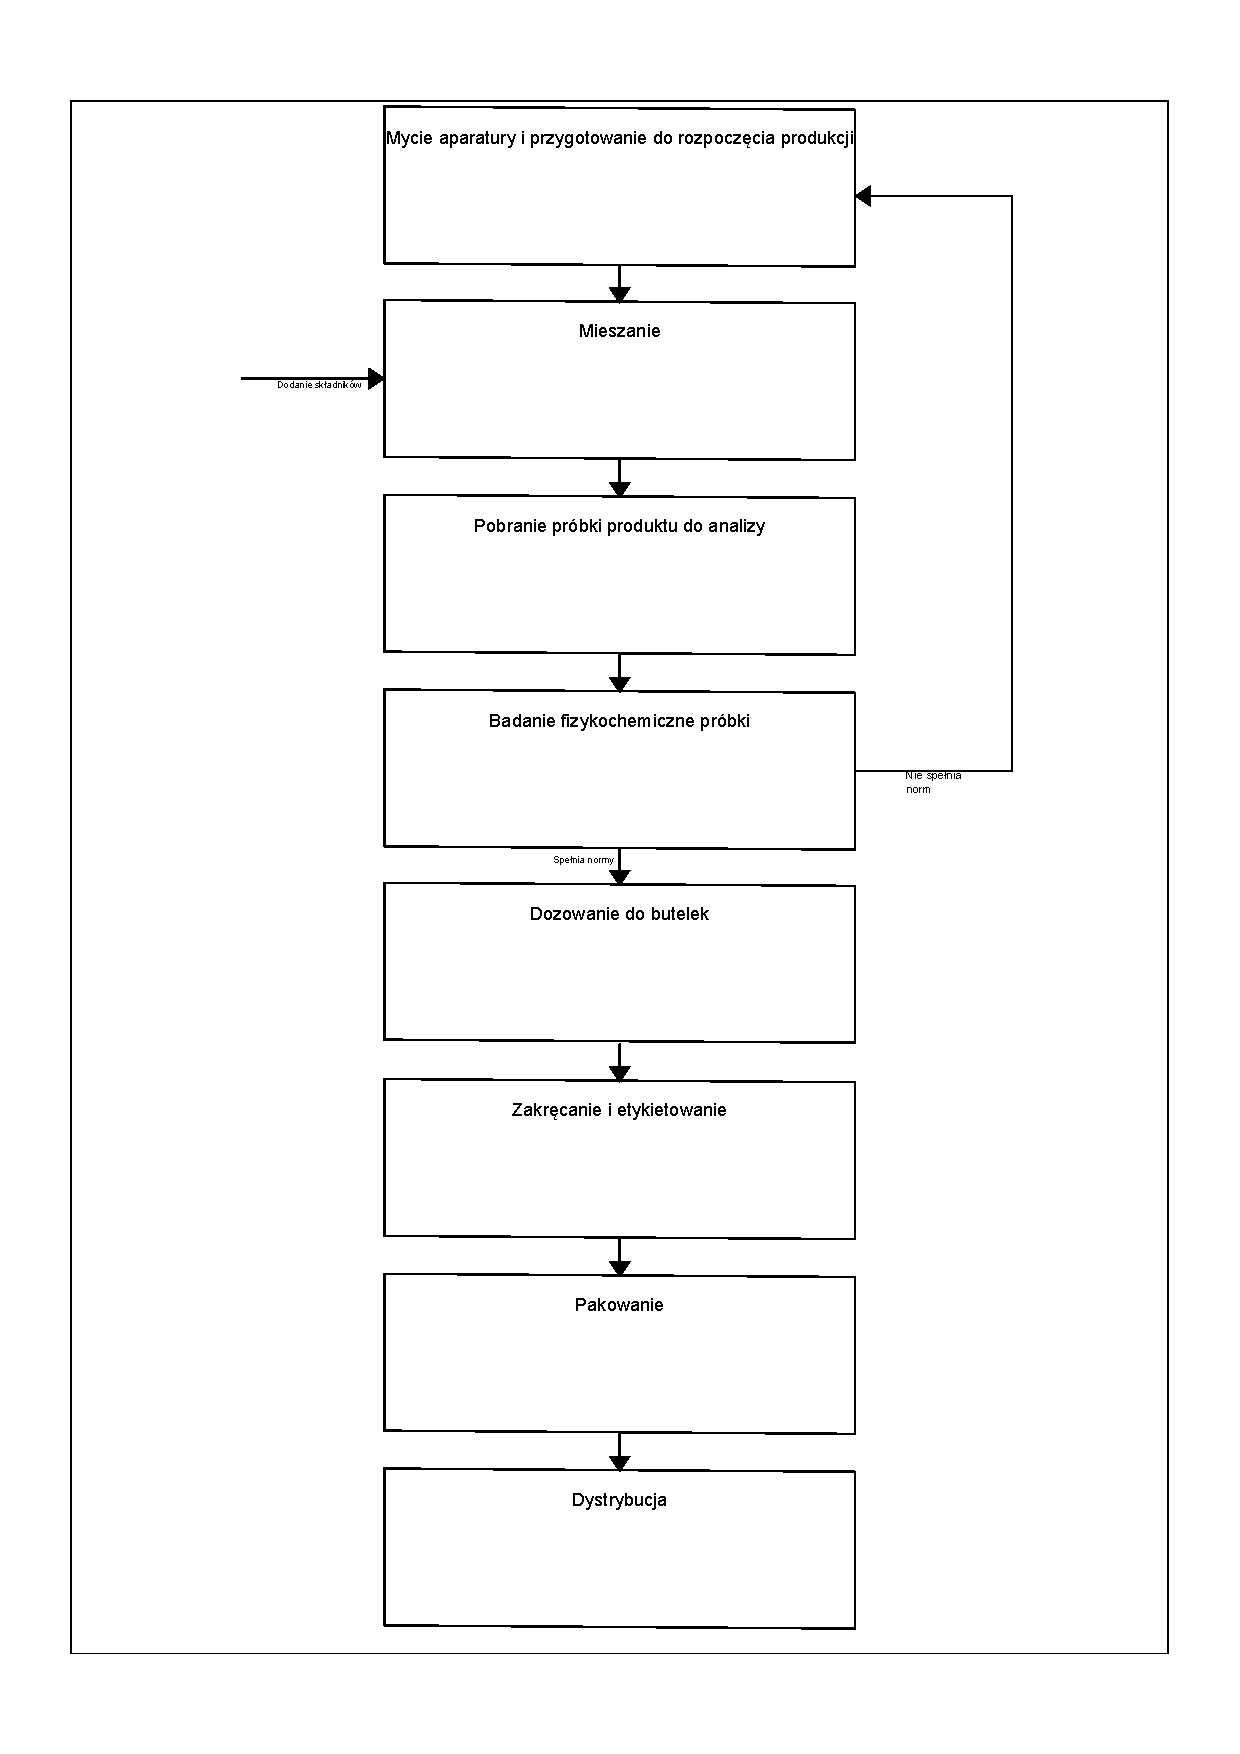
\includegraphics[width=0.9\textwidth]{./sec5/Schemat-blokowy-produkcji-Model.pdf}
\end{figure}


\section{Program i sezonowość produkcji, warianty produkcji w sezonie letnim i zimowym, bilans materiałowy}

Projekt zakłada pracę 5 dni w tygodniu w godzinach 6-22. przez cały rok (z wyłączeniem świąt). Produkowane będą 3 typy odżywek: proteinowa, emolientowa, humektantowa i 2 typy szamponów: ziołowy oraz peelingujący. Wszystkie z tych produktów wytwarzane będą z jednakową intensywnością niezależnie od pory roku. Każdego dnia w zakładzie będzie przebiegać jeden cykl produkcyjny dla każdego typu produktu.

\begin{table}[h]
	\centering
	\caption{Program produkcji}
	\begin{tabular}{lllll}
		\hline
		\textbf{Produkt} & \makecell[l]{\textbf{Produkcja w} \\ \textbf{skali roku [kg]}} & \makecell[l]{\textbf{Produkcja w} \\ \textbf{skali roku [hl]}} & \makecell[l]{\textbf{Produkcja na} \\ \textbf{dobę [kg]}} & \makecell[l]{\textbf{Produkcja na} \\  \textbf{dobę [hl]}} \\
		\hline\hline
	Odżywka proteinowa & 150\,000 & 1\,500 & 625,2 & 6,252 \\
	Odżywka emolientowa & 150\,000 & 1\,500 & 625,2 & 6,252 \\
	Odżywka humektantowa & 150\,000 & 1\,500 & 625,2 & 6,252 \\
	Szampon ziołowy & 330\,000 & 3\,300 & 1\,375 & 13,75 \\
	Szampon wzbogacony & 330\,000 & 3\,300 & 1\,375 & 13,75 \\
	\hline
	\end{tabular}
\end{table}

\begin{table}[h]
	\centering
	\caption{Zapotrzebowanie na surowce do produkcji szampon}
	\begin{tabular}{llll}
		\hline
		\textbf{Produkt} & \textbf{Surowiec} & \makecell[l]{\textbf{Zapotrzebowanie} \\ \textbf{dobowe [kg]}} & \makecell[l]{\textbf{Zapotrzebowanie} \\ \textbf{roczne [kg]}} \\
		\hline\hline
		\multirow{12}{*}{Szampon ziołowy} & Woda & 1090,375 & 261690 \\
		 & Sodium Coco Sulfate & 137,5 & 33000 \\
		 & Rubus idaeus L. Leaf Extract & 110 & 26400 \\
		 & Urtica dioica L. Leaf Extract & 96,25 & 23100 \\
		 & Coco-Glucoside & 71,5 & 17160 \\
		 & Cocamidopropyl Betaine & 55 & 13200 \\
		 & Thymus vulgaris L Leaf Extract & 45,375 & 10890 \\
		 & Sodium Benzoate & 34,375 & 8250 \\
		 & Guar Hydroxypropyltrimonium Chloride & 27,5 & 6600 \\
		 & Citric Acid & 24,75 & 5940 \\
		 & Sodium Chloride & 13,75 & 3300 \\
		 & Tocopherol & 2,75 & 660 \\
		\hline
		\multirow{12}{*}{Szampon peelingujący} & Woda & 660 & 158400 \\
		 & Coffea arabica L. Bean Grind & 204,875 & 49170 \\
		 & Sodium Coco Sulfate & 185,625 & 44550 \\
		 & Glycerin & 68,75 & 16500 \\
		 & Prunus Amygdalus Dulcis (Sweet Almond) Oil & 55 & 13200 \\
		 & Cocamidopropyl Betaine & 55 & 13200 \\
		 & Coco-Glucoside & 55 & 13200 \\
		 & Citric Acid & 48,125 & 11550 \\
		 & Guar Hydroxypropyltrimonium Chloride & 26,125 & 6270 \\
		 & Sodium Benzoate & 15,125 & 3630 \\
		 & Sodium Chloride & 13,75 & 3300 \\
		 & Tocopherol & 1,375 & 330 \\
		 \hline
	\end{tabular}
\end{table}


\begin{table}[h]
	\centering
	\caption{Zapotrzebowanie na surowce do produkcji odżywek}
	\begin{tabular}{llll}
		\hline
		\textbf{Produkt} & \textbf{Surowiec} & \makecell[l]{\textbf{Zapotrzebowanie} \\ \textbf{dobowe [kg]}} & \makecell[l]{\textbf{Zapotrzebowanie} \\ \textbf{roczne [kg]}} \\
		\hline\hline
		\multirow{14}{*}{Odżywka proteinowa} & Woda & 306,348 & 73500 \\
		 & Cetearyl Alkohol & 137,544 & 33000 \\
		 & Quercus robur L. Bark Extract & 43,764 & 10500 \\
		 & Glycerin & 31,26 & 7500 \\
		 & Wheat Amino Acids & 28,134 & 6750 \\
		 & Behentrimonium Chloride & 25,008 & "6000 \\
		 & Polyglyceryl-3 PCA & 12,504 & 3000 \\
		 & Potassium Sorbate & 12,504 & 3000 \\
		 & Sodium Benzoate & 12,504 & 3000 \\
		 & Dehydroacetic Acid & 6,252 & 1500 \\
		 & Citric Acid & 5,6268 & 1350 \\
		 & Lactic Acid & 1,2504 & 300 \\
		 & Linalool & 1,2504 & 300 \\
		 & Tetrasodium EDTA & 1,2504 & 300 \\
		\hline
		\multirow{14}{*}{Odżywka emolientowa} & Woda & 250,08 & 60000 \\
		 & Butyrospermum Parkii (Shea Butter) & 87,528 & 21000 \\
		 & Vitis labrusca fruit extract & 59,394 & 14250 \\
		 & Argan Oil & 53,142 & 12750 \\
		 & Black Cumin Oil & 50,016 & 12000 \\
		 & Cetearyl Alcohol & 43,764 & 10500 \\
		 & Macadamia Ternifolia Seed Oil & 25,008 & 6000 \\
		 & Brassica Oleracea Italica Seed Oil & 18,756 & 4500 \\
		 & Prunus Domestica (Plum) Seed Oil & 18,756 & 4500 \\
		 & Camellia Japonica Seed Oil & 12,504 & 3000 \\
		 & Benzoic Acid & 1,8756 & 450 \\
		 & Dehydroacetic Acid & 1,8756 & 450 \\
		 & Phenoxyethanol & 1,2504 & 300 \\
		 & Linalool & 1,2504 & 300 \\
		\hline
		\multirow{9}{*}{Odżywka humektantowa} & Woda & 287,592 & 69000 \\
		 & Aloe Barbadensis (Aloe Vera) Leaf Juice & 125,04  & 30000 \\
		 & Cetearyl Alcohol & 62,52 & 15000 \\
		 & Glycerin & 56,268 & 13500 \\
		 & Persea Gratissima Oil & 43,764 & 10500 \\
		 & Behentrimonium Chloride & 31,26 & 7500 \\
		 & Polyglyceryl-3 PCA & 12,504 & 3000 \\
		 & Benzoic Acid & 3,126 & 750 \\
		 & Dehydroacetic Acid & 3,126 & 750 \\
		 \hline
	\end{tabular}
\end{table}

\textbf{Przykładowe obliczenia:}

Woda (odżywka proteinowa):

\begin{equation}
	0,147 \frac{kg}{butelka} \cdot 2\,084 \frac{butelek}{doba} = 306.348kg; \qquad
	0,147 \frac{kg}{butelka} \cdot 500\,000 \frac{butelek}{rok} = 73\,500
\end{equation}

Tocopherol (szampon ziołowy):
\begin{equation}
	1 \frac{g}{butelka} \cdot 2\,750 \frac{butelek}{doba} = 2.75 kg; \qquad
	1 \frac{g}{butelka} \cdot 660\,000 \frac{butelek}{rok} = 660kg
\end{equation}



\section{Spis maszyn i urządzeń}

\begin{table}[h]
\centering
\begin{scriptsize}
	\caption{Spis maszyn i urządzeń}
	\begin{tabular}{*{12}{|l}|}
		\hline
		\multirow{3}{*}{Lp.} & \multirow{3}{*}{\makecell[l]{Liczba \\ maszyn}} & \multirow{3}{*}{\makecell[l]{Nazwa \\ urządzenia}} & \multirow{3}{*}{\makecell[l]{Typ, firma, \\ producent}} & \multirow{3}{*}{Wydajność} & \multirow{3}{*}{\makecell[l]{Poje--\\mność \\ $[\mathrm{l}]$}} & \multicolumn{3}{l|}{\makecell[l]{Gabaryty \\ {[mm]}}} & \multirow{3}{*}{\makecell[l]{Masa \\ urządzenia \\ {[kg]}}} & \multirow{3}{*}{\makecell[l]{Zużycie \\ mocy \\ {[$kW/db$]}}} & \multirow{3}{*}{Uwagi} \\
		\cline{7-9}
		 &  &  &  &  &  & \makecell[l]{szer--\\okość} & \makecell[l]{dłu--\\gość} & \makecell[l]{wyso--\\kość} &  &  &  \\
		 \hline
		1. & 2 & \makecell[l]{Zbiornik na \\ wodę \\ destylowaną} & \makecell[l]{\textsf{Czysta Woda} \\ \textsf{Śląsk}, DPPL \\ (IBC) typu \\ mauzer} &  & 1000 & 1000 & 1000 & 1200 & 20 &  &  \\
		\hline
		2. & 2 & \makecell[l]{Pompa do \\ wody} & \makecell[l]{\textsf{Speroni} \\ \textsf{CAM80}} & 50 l/min &  & 200 & 445 & 210 & 25 & 1 & \makecell[l]{Zużycie mocy obliczone \\ dla obydwu urządzeń} \\
		\hline
		3. & 1 & Mieszalnik & \textsf{ZRJ-1500} & 600 l/h & 1500 & 4100 & 4000 & 3750 & 350 & 105 &  \\
		\hline
		4. & 1 & Mieszalnik & \textsf{ZRJ-750} & 300 l/h & 750 & 3200 & 3800 & 3050 & 250 & 60 &  \\
		\hline
		5. & 2 & \makecell[l]{Pompa \\ dozująca} & \textsf{EURALCA} & 700l/h &  & 250 & 350 & 400 & 22 & 1 & \makecell[l]{Zużycie mocy obliczone \\ dla obydwu urządzeń} \\
		\hline
		\multirow{9}{*}{6.} & \multirow{9}{*}{2} & \multirow[m]{9}{*}{\makecell[l]{Maszyna do \\ napełniania \\ płynów, \\ zakręcania \\ butelek i \\ etykietowania}} & \makecell[l]{Napełniarka \\ rzędowa \\ \textsf{AT-L16} \\ typ \textsf{NPACK}} & \makecell[l]{2500 \\ butelek/h} &  & 900 & 2000 & 2100 & 400 & 1,6 & \makecell[l]{Zużycie mocy obliczone \\ dla obydwu urządzeń} \\
		\cline{4-12}
		 & & & \makecell[l]{Obrotowa \\ maszyna \\ wlotowa \\ \textsf{NPACK-J}} & \makecell[l]{3000\\ butelek/h} &  & 960 & 2400 & 2100 & 550 & 3,2 & \makecell[l]{Zużycie mocy obliczone \\ dla obydwu urządzeń} \\
		\cline{4-12}
		& & & \makecell[l]{Maszyna do \\ etykietowania \\ butelek \\ \textsf{NPACK-TB-YP}} & \makecell[l]{3000 \\ butelek/h} &  & 650 & 1700 & 1300 & 120 & 0,4 & \makecell[l]{Zużycie energii obliczone \\ dla obydwu urządzeń} \\
		\hline
	\end{tabular}
\end{scriptsize}
\end{table}


\section{Rysunki schematyczne linii aparaturowych}

\begin{figure}[h]
	\centering
	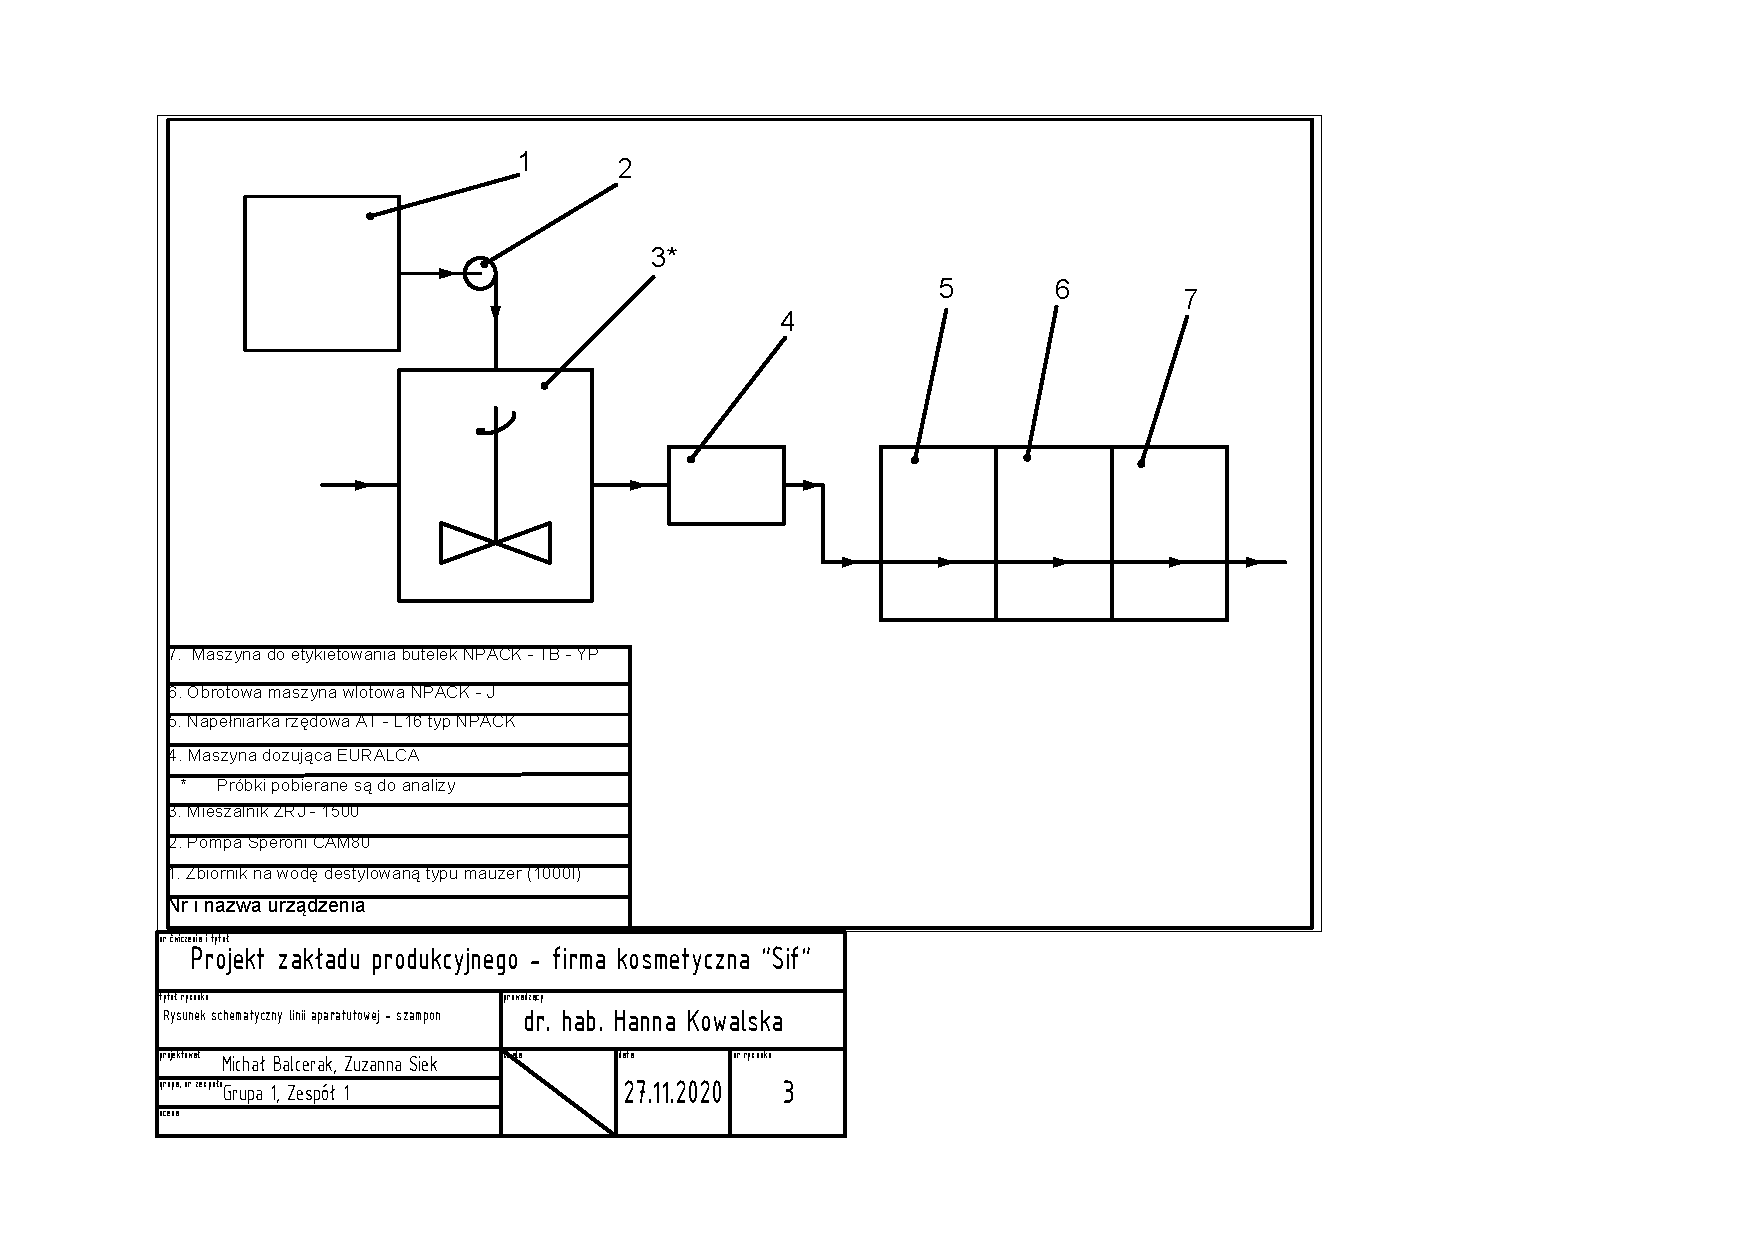
\includegraphics[width=\textwidth]{./sec8/linia_szampony.pdf}
	\caption{Schemat linii aparaturowej produkcji szamponów}
\end{figure}

\begin{figure}[h]
	\centering
	\includegraphics[width=\textwidth]{./sec8/linia_odżywki.pdf}
	\caption{Schemat linii aparaturowej produkcji odżywki}
\end{figure}


\section{Bilans opakowań i materiałów pomocniczych}

Kosmetyki rozlewane do butelek wykonanych z materiału bio-PET pochodzącego w 100\% z recyklingu, stworzonego na bazie trzciny cukrowej.

\begin{figure}[h]
	\centering
	\begin{subfigure}[t]{0.45\textwidth}
	\centering
	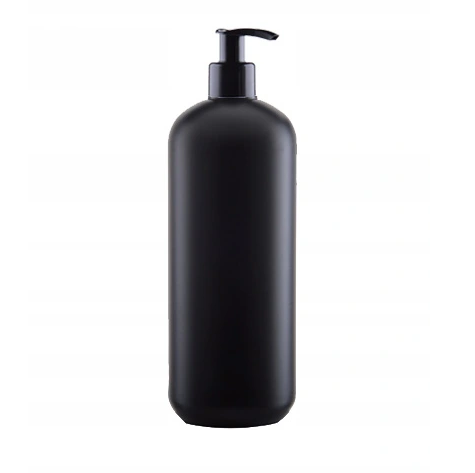
\includegraphics[width=\textwidth]{./sec9/butelka1.png}
		\caption{Dozownik w formie pompki; pojemność: 500\,ml; wymiary 7,4\,cm x 7,4\,cm x 18,6\,cm; waga 35\,g; kolor czarny; ilość w kartonowym opakowaniu zbiorczym 100 sztuk\protect\footnote{\url{https://allegro.pl/oferta/butelka-z-\-dozownikiem-do-zelu-mydla-pompka-500ml-9708856613?bi_s=ads&bi_m=showitem\%3Aactive&bi_c=NjRhY2JkMDYtYzc5MS00MjkxLTlmZDAtM2FhZGI5MzBiMzFjAA&bi_t=ape&referrer=proxy&emission_unit_id=b357113d-ff81-4cbf-93b9-39d19bdc982c}}}
	\end{subfigure}
	\hfill
	\begin{subfigure}[t]{0.45\textwidth}
	\centering
	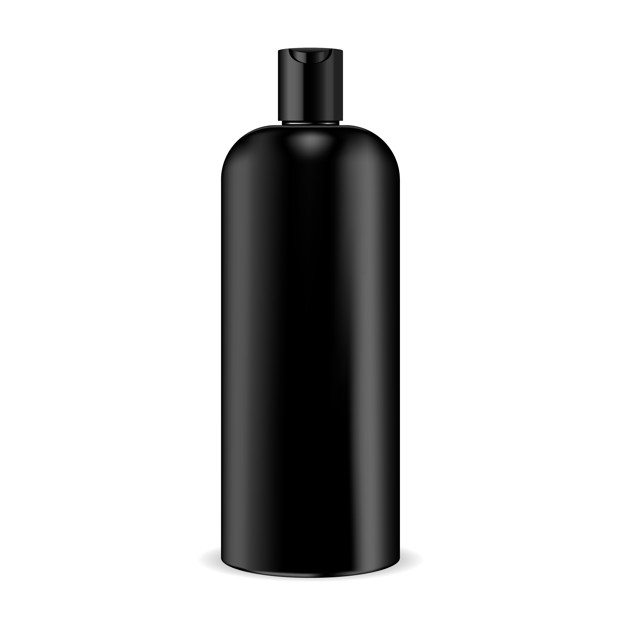
\includegraphics[width=\textwidth]{./sec9/butelka2.jpg}
		\caption{Zamknięcie typu disc cap; pojemność: 300\,ml; wymiary 16,5\,cm x 6,4\,cm x 6,4\,cm; waga 21\,g; kolor czarny; ilość w kartonowym opakowaniu zbiorczym 125 sztuk\protect\footnote{\url{https://www.freepik.com/premium-vector/cosmetic-shampoo-black-bottle-mockup_4188953.html}}}
	\end{subfigure}
	\caption{Butelki na (a) szampony i (b) odżywki}
\end{figure}

\begin{table}[h]
	\centering
	\caption{Etykiety wykonane z papieru metalizowanego. Zapotrzebowanie}
	\begin{tabular}{lllll}
		\hline
		\textbf{Produkt} & \textbf{Produkcja roczna} & \makecell[l]{\textbf{Zapotrzebowanie} \\ \textbf{dzienne}} & \makecell[l]{\textbf{Zapotrzebowanie} \\  \textbf{tygodniowe}} & \makecell[l]{\textbf{Zapotrzebowanie} \\ \textbf{miesięczne}} \\
		\hline\hline
		Odżywka proteinowa & 500 tys. butelek 300ml & \multirow{3}{*}{\makecell[l]{6250 sztuk \\ 50 kartonów butelek}} & \multirow{3}{*}{\makecell[l]{31250 sztuk \\ 250 kartonów butelek}} & \multirow{3}{*}{\makecell[l]{131250 sztuk \\ 1050 kartonów butelek}} \\
		Odżywka emolientowa & 500 tys. butelek 300ml & & & \\
		Odzywka humektantowa & 500 tys. butelek 300ml & & & \\
		\cline{3-5}
		Szampon ziołowy & 660 tys. butelek 500ml & \multirow{2}{*}{\makecell[l]{5500 sztuk\\ 55 kartonów butelek}} & \multirow{2}{*}{\makecell[l]{27500 sztuk \\ 275 kartonów butelek}} & \multirow{2}{*}{\makecell[l]{115500 sztuk \\ 1155 kartonów butelek}} \\
		Szampon peelingujący & 660 tys. butelek 500ml \\
		\hline
	\end{tabular}
\end{table}



\section{Normy i akty prawne}

\begin{itemize}
	\item Prawo budowlane
	\item Prawo ochrony środowiska
	\item Prawo energetyczne
	\item USTAWA o planowaniu i zagospodarowaniu przestrzennym
	\item USTAWA o efektywności energetycznej
	\item Rozporządzenie w sprawie ogólnych przepisów bezpieczeństwa i higieny pracy
	\item Prawo wodne
	\item Dyrektywa w sprawie monitorowania temperatur w środkach transport
	\item Kosmetyk naturalny musi być wyprodukowany zgodnie ze standardem GMP (Good Manufacturing Practice – Dobra Praktyka Produkcyjna). Standard GMP określa norma ISO 22716:2007, która precyzuje wymagania dotyczące m.in. personelu, pomieszczeń czy urządzeń stosowanych do produkcji kosmetyków.
	\item Produkt, który ma zostać wprowadzony na rynek, należy notyfikować w systemie Cosmetic Products Notification Portal (CPNP), bazie zbierającej informacje na temat kosmetyków wprowadzonych do obrotu na terenie Unii Europejskiej.
	\item Rozporządzenie 1223/2009, dot. informacji na opakowaniu produktu kosmetycznego
	\item Rozporządzenie 655/2013 dot. deklaracji marketingowych
	\item Norma 16128-1:2016 oraz 16128-2:2017 określa definicje naturalnych i organicznych składników oraz prezentuje metodologię obliczania indeksów naturalności, naturalnego pochodzenia oraz organiczności i organicznego pochodzenia.
	\item Rozporządzenie 1223/2009 wymaga, aby wszystkie informacje dotyczące bezpieczeństwa zostały zawarte w raporcie bezpieczeństwa produktu kosmetycznego.
	\item Rozporządzenie 655/2013/ WE [2, 9].  ustawa opakowaniowa
	\item Pozwolenie wodno – prawne
	\item Ustawa z dnia 4 października 2018 r. o produktach kosmetycznych
	\item Ustawa z dnia 30 marca 2001 r. o kosmetykach
	\item Rozporządzenie Ministra Zdrowia z dnia 20 lutego 2019 r. w sprawie Ośrodka administrującego Systemem Informowania o Ciężkich Działaniach Niepożądanych Spowodowanych Stosowaniem Produktów Kosmetycznych.
	\item Rozporządzenie Ministra Zdrowia z dnia 28 lutego 2019 r. w sprawie określenia wzorów wniosków oraz zaświadczeń związanych z wykazem zakładów wytwarzających produkty kosmetyczne.
	\item Rozporządzenie Ministra Zdrowia z dnia 28 lutego 2019 r. w sprawie ośrodka uprawnionego do dostępu do informacji o produkcie kosmetycznym.
	\item Rozporządzenie Ministra Zdrowia z dnia 19 marca 2020 r. w sprawie metod oznaczeń próbek niezbędnych do kontroli bezpieczeństwa produktów kosmetycznych.
	\item Rozporządzenie Ministra Opieki Społecznej z dnia 18 stycznia 1939 r. s prawie  dozoru nad wyrobem i obiegiem środków kosmetycznych.
	\item Zarządzenie Ministrów: Przemysłu Rolnego i Spożywczego, Przemysłu Drobnego i Rzemiosła, Handlu Wewnętrznego oraz Zdrowia w sprawie unormowania produkcji i dystrybucji wyrobów kosmetycznych.
	\item Dyrektywa Komisji 95/17/WE z dnia 19 czerwca 1995 r. ustanawiająca szczegółowe zasady stosowania dyrektywy Rady 76/768/EWG w odniesieniu do nieumieszczania jednego lub kilku składników w wykazie używanym do etykietowania produktów kosmetycznych.
	\item Siódma Dyrektywa Komisji 96/45/WE z dnia 2 lipca 1996 r. odnosząca się do metod analizy niezbędnych do kontroli składu produktów kosmetycznych.
	\item k.p.a. – ustawa z dnia 14 czerwca 1960 r. – Kodeks postępowania administracyjnego (t. jedn. Dz. U. 2018, poz. 2096)
	\item u.i.h. - ustawa z dnia 15 grudnia 2000 r. o Inspekcji Handlowej (t. jedn. Dz. U. 2018, poz. 1930 z późn. zm.)
	\item u.k. – ustawa z dnia 30 marca 2001 r. o kosmetykach (t. jedn. Dz. U. 2013, Nr 475 z późn. zm.)
	\item u.b.p. - ustawa z dnia 12 grudnia 2003 r. o ogólnym bezpieczeństwie produktów (t. jedn. Dz.U. 2016, poz. 2047) 41
	\item u.o.k.k. – ustawa z dnia 16 lutego 2007 roku o ochronie konkurencji i konsumentów (t. jedn. Dz.U.2018, poz.798) u.p.k. – ustawa z dnia 4 października 2018 r. o produktach kosmetycznych (Dz.U. 2018, poz. 2227)
	\item u.p.n.p.r. – ustawa z dnia 23 sierpnia 2007 roku o przeciwdziałaniu nieuczciwym praktykom rynkowym (t. jedn. Dz.U.2017, poz.2070)
	\item u.p.p. – ustawa z dnia 26 stycznia 1984 roku – Prawo prasowe (t. jedn. Dz.U.2018, poz.1914)
	\item u.z.n.k. – ustawa z dnia 16 kwietnia 1993 roku o zwalczaniu nieuczciwej konkurencji (t. jedn. Dz.U.2018, poz.419)
	\item RODO - Rozporządzenie Parlamentu Europejskiego i Rady (UE) 2016/679 z dnia 27 kwietnia 2016 r. w sprawie ochrony osób fizycznych w związku z przetwarzaniem danych osobowych i w sprawie swobodnego przepływu takich danych oraz uchylenia dyrektywy 95/46/WE (ogólne rozporządzenie o ochronie danych); Dz. Urz. UE L 119 z 04.05.2016, s. 1.
	\item Rozporządzenie 1223/2009 – Rozporządzenie Parlamentu Europejskiego i Rady z dnia 30 listopada 2009 r. dotyczące produktów kosmetycznych (Dz. Urz. L 342 z 22.12.2009, s. 59-209)
	\item Decyzja wykonawcza Komisji z dnia 25 listopada 2013 r. w sprawie wytycznych dotyczących załącznika I do rozporządzenia Parlamentu Europejskiego i Rady (WE) nr 1223/2009 dotyczącego produktów kosmetycznych (Dz.U. L z 2013, poz. 315, s. 82—104)
	\item Podręcznik Grupy Roboczej ds. Produktów Kosmetycznych (Podgrupy ds. produktów z pogranicza) dotyczący stosowania Rozporządzenia Parlamentu Europejskiego i Rady (WE) nr 1223/2009 z dnia 30 listopada 2009 r. dotyczącego produktów kosmetycznych (wersja 1.0 listopad 2013 r.)
	\item Rozporządzenie 655/2013/WE określające wspólne kryteria dotyczące uzasadniania oświadczeń stosowanych w związku z produktami kosmetycznymi oraz wytyczne do tego rozporządzenia
	\item Sprawozdanie Komisji Dla Parlamentu Europejskiego i Rady z dnia 19.9.2016 r. na temat oświadczeń o produktach sporządzanych na podstawie wspólnych kryteriów w branży kosmetycznej COM/2016/0580 final
	\item Rozporządzenie Ministra Zdrowia z dnia 16 czerwca 2003 r. w sprawie określenia kategorii produktów będących kosmetykami (Dz.U. z 2003 poz. 125, Nr 1168)
	\item Kodeks Etyki Reklamy opracowany przez Związek Stowarzyszeń Rady Reklamy,
	\item Zasady Przewodnie Stowarzyszenia Cosmetics Europe w zakresie Reklamy i Oświadczeń Marketingowych,
	\item Karta Odpowiedzialnej Reklamy i Komunikacji Marketingowej Stowarzyszenia Cosmetics Europe.
\end{itemize}


\section{Warunki magazynowania surowców, produktów i niektórych materiałów pomocniczych}

\textbf{Aqua (Woda)}: będzie przechowywana w temperaturze pokojowej w paletopojemnikach na hali produkcyjnej niedaleko mieszalnik\vspace{\baselineskip}

\textbf{Składniki do produkcji szamponów i odżywek:}
\begin{itemize}
	\item Sodium Coco Sulfate
	\item Coco-Glucoside
	\item Coffea arabica L. Bean Grind
	\item Sodium Benzoate
	\item Rubus idaeus L. Leaf Extract
	\item Cocamidopropyl Betaine
	\item Urtica dioica L. Leaf Extract
	\item Prunus Amygdalus Dulcis (Sweet Almond) Oil
	\item Guar Hydroxypropyltrimonium Chloride
	\item Thymus vulgaris L Leaf Extract
	\item Sodium Chloride
	\item Tocopherol
	\item Cetearyl Alcohol
	\item Glycerin
	\item Behentrimonium Chloride
	\item Sodium Benzoate
	\item Citric Acid
	\item Benzoic Acid
	\item Dehydroacetic Acid
	\item Phenoxyethanol
	\item Tetrasodium EDTA
	\item Lactic Acid
	\item Linalool
	\item Potassium Sorbate
	\item Camellia Japonica Seed Oil
	\item Prunus Domestica (Plum) Seed Oil
	\item Brassica Oleracea Italica Seed Oil
	\item Polyglyceryl-3 PCA
	\item Macadamia Ternifolia Seed Oil
	\item Black cumin oil
	\item Argan oil
	\item Vitis labrusca fruit extract
	\item Butyrospermum Parkii (Shea Butter)
	\item Aloe Barbadensis (Aloe Vera) Leaf Juice
	\item Persea Gratissima Oil
	\item Quercus robur L. Bark Extract
	\item Wheat Amino Acids
\end{itemize}

Będą przechowywane w szczelnie zamkniętych opakowaniach w magazynie znajdującym się niedaleko hali produkcyjnej. Na magazynie będzie utrzymywana temperatura ok 18C, wilgotność powietrza 35\% oraz będzie utrzymywane zacienienie. Pomieszczenie to będzie dobrze wentylowane. \vspace{\baselineskip}

\textbf{Produkty (szampony oraz odżywki):}

Będą przechowywane w tym samym magazynie (takie same parametry temperatury, wilgotności i dostępu do światła), co składniki do ich produkcji. Przechowywane w pudełkach ułożonych na paletach. \vspace{\baselineskip}

\textbf{Środki myjące:}

Będą magazynowane w małym pomieszczeniu przeznaczonym specjalnie na środki i sprzęt do mycia, w temperaturze pokojowej. Pomieszczenie będzie zlokalizowane blisko hali produkcyjnej, aby był łatwy dostęp do środków myjących.


\section{Warunki magazynowania surowców, produktów i niektórych materiałów pomocniczych}

Ze względów funkcjonalnych jak i higienicznych, magazyn główny firmy \textsf{Sif} będzie podzielony na trzy części:
\begin{itemize}
	\item magazyn surowców do produkcji;
	\item magazyn gotowego produktu;
	\item magazyn pustych opakowań
\end{itemize}

Ponadto funkcję magazynu będzie pełniła część powierzchni hali produkcyjnej, na której będą znajdowały się paletopojemniki z wodą, a także część przeznaczona na przechowywanie środków czystości.

Magazyn będzie znajdował się niedaleko hali produkcyjnej, co zapewni dogodny dostęp do serowca podczas przygotowywania produktu oraz jego sprawne zmagazynowanie po pokończonym procesie.

Założenia dotyczące magazynowania:
\begin{itemize}
	\item Magazyn będzie wyposażony w regały paletowe rzędowe pozwalające na składowanie towarów spaltyzowanych i niespaletyzowanych. Pojedynczy regł ma długość 6.6\,m, szerokość 2\,m oraz 2 (dwa) poziomy. Pozwala na składowanie palet po obydwu stronach w ilości 10 sztuk na jednym poziomie czyli 20 sztuk na wszystkich poziomach łącznie
	\item Wysokość magazynu -- 6\,m
	\item 70\% magazynu stanowi pojedyncza powierzchnia składowań, 30\% powierzchnia strefy buforowej przy rampach, przeznaczona do tymczasowego składowania rozładowywanych surowców lub produktów przygotowywanych do wysyłki
	\item Korytarze pomiędzy regałami, a także ścianą i regałami będą wynosiły około 4\,
\end{itemize}\vspace{\baselineskip}

\textbf{Magazyn na surowce}

Obliczenia dotyczące liczby jednorazowo składowanych europalet (na przykładzie firmy \textsf{TRB Natural Extraxt}):

Dostarczanych będzie 170 sztuk worków o pojemności 25\,kg jednego surowca oraz 77 sztuk drugiego. Na jednej europalecie może być składowane 35 worków o pojemność 25\,kg
\[
	5\,\mathrm{szt.} \cdot 7\,\text{ poziomów}
\]
Zatem łącznie dostarczanych będzie 7 europalet
\[
	\frac{170}{35} + \frac{77}{35} = 7
\]
Liczba europalet dostarczanych przez pozostaję firmy została wyznaczona w analogiczny sposób i wynosi dla firmy:
\begin{itemize}
	\item \textsf{OQEMA} -- 33 sztuk europalet/paletopojemników
	\item \textsf{Distripark} -- 10 sztuk europalet
	\item \textsf{CIECH S.A.} -- 1 sztuka europalety
	\item \textsf{Sigma-Aldrich} -- 4 sztuki europalet
	\item \textsf{PK Components} -- 10 sztuk europalet
	\item \textsf{Supreme Gums} -- 2 sztuki europalet
\end{itemize}

Liczba jednorazowo składowanych europalet w magazynie surowców wynosi 67.\vspace{\baselineskip}

Obliczenia dotyczące powierzchni magazynów:
\begin{itemize}
	\item Pojedynczy regał ma miejsca na 20 palet, a magazyn musi pomieścić 67 palet
	\item Zakładamy, że 10\% lokalizacji zostaję wolnych, aby zapewnić płynność pracy magazynu w przypadku spiętrzeń przepływu towaru, zatem liczba palet mieszczących się w 1 regale wynosi 18 ($20 \cdot 0.9$)
	\item Magazym musi zawierać 4 regały (67/18 = 3.7 = 4)
	\item Pomiędzy ścianami a regałem oraz pomiędzy regałami są korytarze 4\,m, jest 5 korytarzy wzdłuż ścian krótszych -- szerokość, oraz 2 wzdłuż ścian dłuższych -- długość.
	\item Regały ustawione są wzdłuż ścian krótszych (szerokość)
	\item Szerokość regału to 2\,m, a długość to 6.6\,m
	\item Długość magazynu to $5 \cdot 4\mathrm{m} + 4 \cdot 2\mathrm{m} = 28\mathrm{m}$
	\item Szerokość magazynu to $2\cdot 4\mathrm{m} + 6.6\mathrm{m} = 15\mathrm{m}$
	\item Powierzchnia składowania to $15\mathrm{m} \cdot 28\mathrm{m} = 420\mathrm{m}$
	\item Powierzchnia składowania stanowi 70\% zatem doliczając powierzchnię strefy buforowej uzyskujemy łączną powierzchnię magazynu wynoszącą $\mathbf{600\mathrm{m^{3}}}$
\end{itemize}\vspace{\baselineskip}

\textbf{Magazyn pustych opakowań}:
\begin{itemize}
	\item Musi pomieścić miesięczny zapas opakowań oraz etykiet, czyli 147 palet
	\item Do tego celu posłuży 8 regałów
	\item Długość magazynu -- 44\,m
	\item Szerokość magazynu -- 15\,m
	\item Powierzchnia składowania -- 660\,$\mathrm{m^{2}}$
	\item Powierzchnia składowani stanowi 70\% zatem doliczając powierzchnię strefy buforowej uzyskujemy łączną powierzchnię magazynu wynoszącą $\mathbf{945m^{2}}$ (długość 63\,m)
\end{itemize}\vspace{\baselineskip}

\textbf{Nagazyn gotowego produktu}:
\begin{itemize}
	\item Musi pomieścić tygodniową produkcję szamponów i odżywek, czyli 26 palet.
	\item Do tego celu posłużą 2 regały.
	\item Długość magazynu: 12',m
	\item Szerokość magazynu: 15',m
	\item Powierzchnia składowania: 180$\mathrm{m^{2}}$
	\item Powierzchnia składowania stanowi 70\% zatem doliczając powierzchnię strefy buforowej uzyskujemy łącznbie powierzchnię magazynu wynoszącą $\mathbf{260m^{2}}$ (długość 17\,m).
\end{itemize}

\begin{table}
	\centering
	\caption{Zestawienie powierzchni}
	\begin{tabular}{cc}
		\hline
		\textbf{Magazyn} & \textbf{Powierzchnia [$\mathbf{m^{3}}$]} \\
		\hline\hline
		Surowców & 600 \\
		Pustych opakowań & 945 \\
		Gotowych produktów & 260 \\
		\textbf{Łącznie} & 1805 \\
		\hline
	\end{tabular}
\end{table}



\section{Środki transportu zewnętrznego i wewnętrznego}

\subsection{Zewnętrzny}

Niezbędne do produkcji składniki będą dostarczane przez zewnętrznych dostawców z wykorzystaniem posiadanych przez nich samochodów dostawczych. Po dotarciu do zakładu składniki będą rozprowadzane do miejsc przeznaczenia przez środki transportu wewnętrznego.\vspace{\baselineskip}

Do dostarczania gotowych produktów do sprzedających je sklepów wykorzystane zostaną samochody dostawcze marki \textsf{Iveco. Model Daily}, który można skonfigurować pod własne potrzeby. Oznacza to, że może on zawierać windę, która znacząco ułatwia zarówno załadunek jak i rozładunek towarów, zwłaszcza w mniejszych sklepach, nie posiadających rampy, oraz jego ładowność maksymalna przy niewielkiej masie (3,5 ton) wynieść może nawet 2700\,kg.

Do celów dostawczych zakładu wykorzystywanych będzie 5 takich samochodów.

\subsection{Wewnętrzny}

W transporcie wewnętrznym potrzebne będą następujące pojazdy:
\begin{itemize}
	\item wózek do przewożenia środków myjących
	\item wózki widłowe do przewożenia palet ze składnikami oraz palet z produktami do samochodów dostawczych
	\item pojazdy dla ochroniarzy
\end{itemize}

Wózki widłowe oraz paletowe zostaną zakupione od firmy \textsf{Wózki Widłowe Blachdeker}. Ich zaletą jest wykorzystanie baterii litowo-jonowej, co umożliwia długo (nawet 8 godzinny) czas pracy na jednym ładowaniu, oraz znacząco skraca czas ładowania. Pozwala to na obniżenie kosztów energii przy jednoczesnym odciążaniu pracowników, którzy nie muszą korzystać z wózków ręcznych. Zaletą wybranej firmy jest oferowany przez nią serwis oraz możliwość leasingu wózków, dzięki czemu koszt ich uzyskania znacznie się obniża.\vspace{\baselineskip}

\textbf{Elektryczny wózek widłowy \textsf{EP L1} udźwig 2000\,kg -- 3 sztuki}

Wózki te będą stosowane przy umieszczaniu dostaw surowców w magazynie, umieszczania tam gotowych produktów oraz przenoszenia gotowych produktów do pojazdów transportujących je do sklepów.\vspace{\baselineskip}

\textbf{Elektryczny wózek paletowy \textsf{EPL 153} udźwig 1\,500\,kg -- 6 sztuk}

Wózki te będą wykorzystywane w obrębie zakładu do transportu składników z magazynu do odpowiednich obszarów hali produkcyjnej (3 sztuki). Innym zastosowaniem dla wózków paletowych będzie wyładowywanie produktów końcowych przy dostawie do sklepów. Będą one przewożone samochodami dostawczymi, by zawsze były do użytku przy wyładowywaniu i rozwożeniu towaru na miejsce.\vspace{\baselineskip}

\textbf{Wózek do sprzątania od firmy \textsf{Numatic} -- 3 sztuki}

Wózki te będą przeznaczone do prac czyszczących, umożliwiając przewożenie środków myjących do obszarów wymagających czyszczenia.\vspace{\baselineskip}

\textbf{Seegway -- \textsf{Airwheel S3} -- 3 sztuki}

Pojazd ten, ze względu na swoją lekkość, łatwość sterowania oraz możliwość szybkiego przyspieszenia stanowi doskonały środek transportu dla ochroniarzy. Można się na nim przemieszczać zarówno w pomieszczeniach jak i na zewnątrz.\vspace{\baselineskip}


\section{Harmonogram pracy maszyn i urządzeń}

Zakład otwierany będzie o 6.00, do 6.30 będzie wszystko uruchamiane i przygotowywane do produkcji, od 6:30 do 7.00 będzie pompowana woda i dodawane składniki do mieszalnika.\vspace{\baselineskip}

Pompa do wody (\textsf{Speroni CAM80}) – 1h dziennie (ok 25 minut na szampon ziołowy, 15 minut na szampon peelingujący, ok 8 minut na odżywkę proteinową, ok 5 minut na odżywkę emolientową, ok 7 minut na odżywkę humektantową)\vspace{\baselineskip}

Mieszalnik (\textsf{ZRJ - 1500}):
\begin{itemize}
	\item praca od 7.00 do 9.30 przy produkcji szamponu ziołowego
	\item praca od 11.30 do 14.00 przy produkcji szamponu peelingującego
	\item łącznie :5 h dziennie przez 5 dni w tygodniu
\end{itemize}\vspace{\baselineskip}

Mieszalnik (\textsf{ZRJ – 750}):
\begin{itemize}
	\item praca od 7.00 do 9.30 przy produkcji odżywki proteinowej
	\item praca od 11.30 do 14.00 przy produkcji odżywki emolientowej
	\item praca od 16.00 do 18.30 przy produkcji odżywki humektantowej
	\item łącznie 7,5 h dziennie przez 5 dni w tygodniu
\end{itemize}\vspace{\baselineskip}

Próbki sprawdzane w laboratorium:
\begin{itemize}
\item od 9.30 do 10.30 szampon ziołowy
\item od 14.00 do 15.00 szampon peelingujący
\item od 9.30 do 10.30 odżywka proteinowa
\item od 14.00 do 15.00 odżywka emolientowa
\item od 18.30 do 19.30 odżywka humektantowa
\end{itemize}\vspace{\baselineskip}

Pompa dozująca (\textsf{EURALCA}):
\begin{itemize}
\item praca od 10.30 do 12.30 przy produkcji szamponu ziołowego
\item praca od 15.00 do 17.00 przy produkcji szamponu peelingującego
\item praca od 10.30 do 11.30 przy produkcji odżywki proteinowej
\item praca od 15.00 do 16.00 przy produkcji odżywki emolientowej
\item praca od 19.30 do 20.30 przy produkcji odżywki humektantowej
\end{itemize}
Łącznie 7h dziennie przez 5 dni w tygodniu ( po 2h na każdy szampon, po 1h na każdą odżywkę)\vspace{\baselineskip}

Maszyna do napełniania płynów, zakręcania butelek i etykietowania:
\begin{itemize}
\item praca od 11.00 do 13.00 przy produkcji szamponu ziołowego
\item praca od 15.30 do 17.30 przy produkcji szamponu peelingującego
\item praca od 11.00 do 12.00 przy produkcji odżywki proteinowej
\item praca od 15.30 do 16.30 przy produkcji odżywki emolientowej
\item praca od 20.00 do 21.00 przy produkcji odżywki humektantowej
\end{itemize}\vspace{\baselineskip}

(Napełniarka rzędowa AT – L16 typ NPACK):

Łącznie 7h dziennie przez 5 dni w tygodniu ( 2h na każdy szampon, 1h na każdą odżywkę)\vspace{\baselineskip}

(Obrotowa maszyna wlotowa NPACK – J):

Łącznie 4h 15 minut dziennie przez 5 dni w tygodniu  (1h na każdy szampon, 45 minut na każdą odżywkę)\vspace{\baselineskip}

(Maszyna do etykietowania butelek NPACK -TB – YP):

Łcznie 4h 15 minut dziennie przez 5 dni w tygodniu  (1h na każdy szampon, 45 minut na każdą odżywkę)\vspace{\baselineskip}



\section{Zużycie wody i poszczególnych czynników energetycznych}

Woda jest dostarczana wodociągami, a woda destylowana jest dostarczana przez firmę zewnętrzną.

Zapotrzebowane na wodę destylowaną do produkcji szamponów i odżywek wynosi 2594.395 i dziennie. Czyli ok. 26\,hl wody destylowanej dziennie. Woda z sieci wodociągowej jest zużywana na mycie urządzeń i powierzchni oraz potrzeby sanitarne.

\begin{figure}[h]
	\centering
	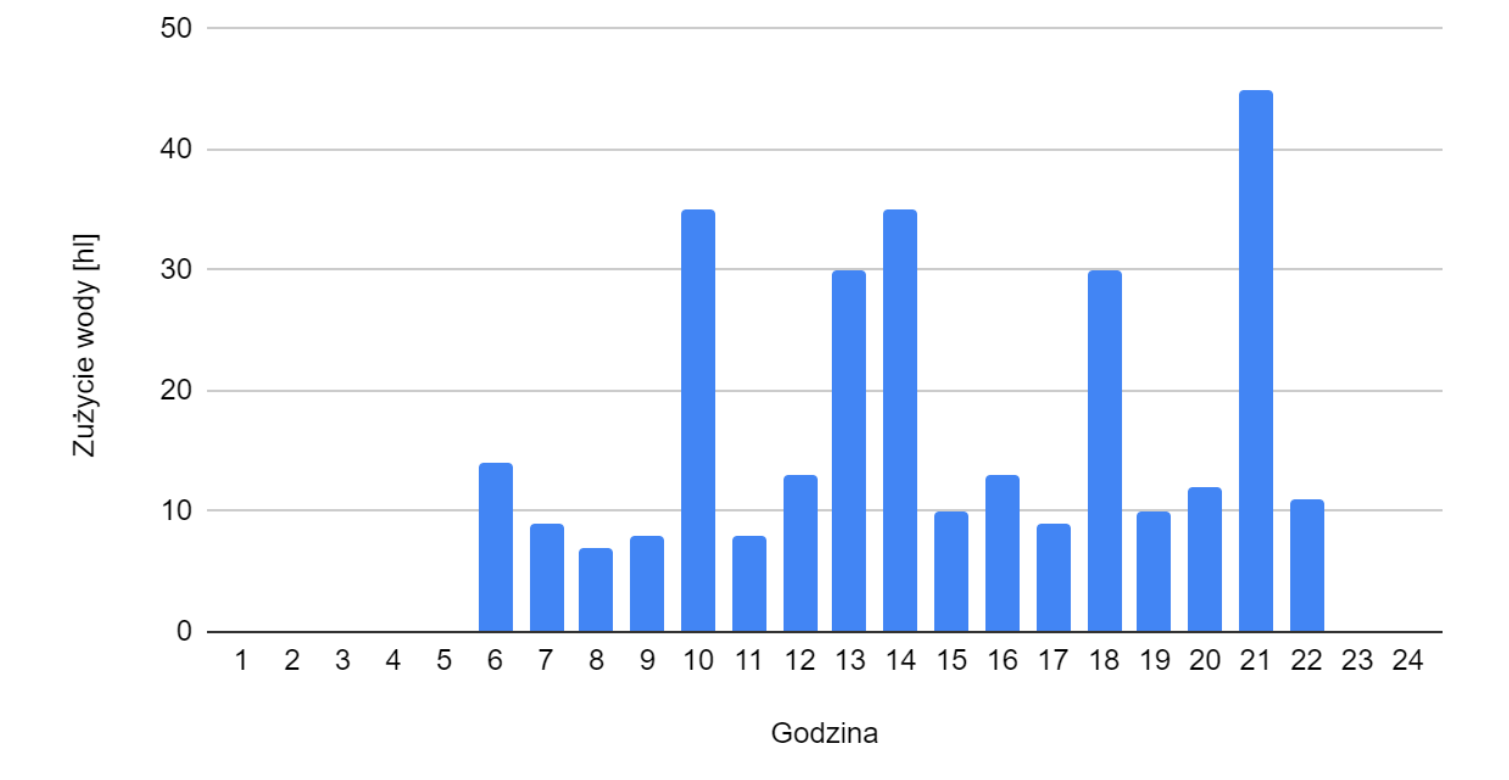
\includegraphics[width=0.8\textwidth]{./sec16/wykres1.png}
	\caption{Harmonogram zużycia wody w ciągu doby}
\end{figure}

Znacznie wyższe zużycie wody w danych godzinach jest spowodowane tym, że w tym czasie następuje mycie urządzeń oraz pompowanie wody potrzebnej do procesu technologicznego. Na koniec zmiany myte są urządzenia oraz podłogi i powierzchnie użytkowe. W godzinach zamknięcia zakładu woda nie jest zużywana. Są to wartości szacunkowe.

Zużycie energii elektrycznej w zakładzie nie jest zróżnicowane sezonowo. Wynika to z faktu, że latem energia zużywana podczas działania klimatyzacji jest porównywalna z energią zużywaną zimą na dogrzewanie pomieszczeń poprzez termowentylatory.  Zarówno latem i zimą energia jest zużywana podczas pracy maszyn ciągu technologicznego oraz oświetlenia zakładu. Średnie godzinowe zużycie energii wynosi 38.58\,kWh. W zakładzie średnio zużywa się 20$\mathrm{\frac{kW}{hl \text{ produkowanego szamponu lub odżywki}}}$.

\begin{figure}[h]
	\centering
	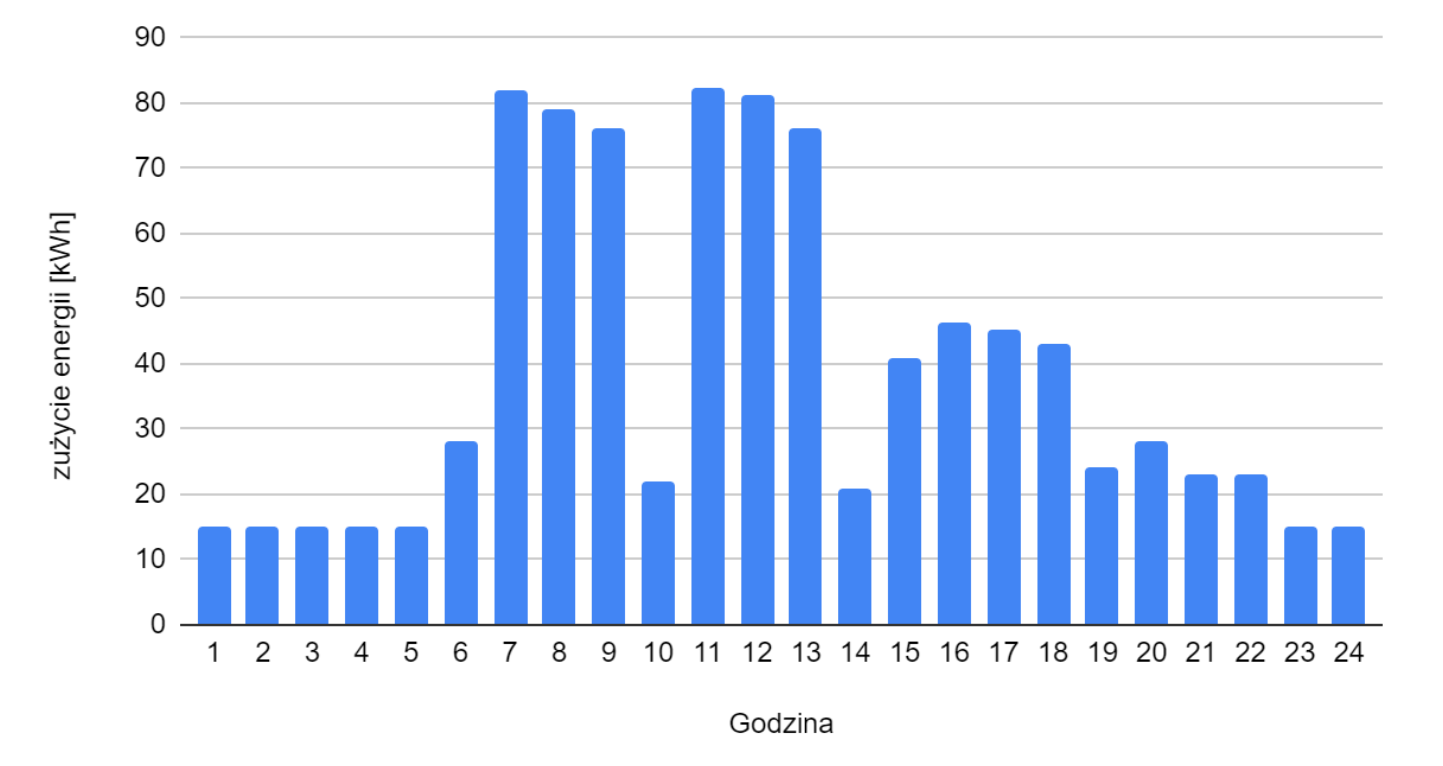
\includegraphics[width=0.8\textwidth]{./sec16/wykres2.png}
	\caption{Harmonogram zużycia energii elektrycznej dla poszczególnych godzin}
\end{figure}

Niskie zużycie energii w godzinach zamknięcia zakładu (22-6) wynika z braku pracy maszyn oraz minimalnego dogrzewania/klimatyzowania pomieszczeń przy jednoczesnym oświetleniu zewnętrznym budynku zakładu. Widoczny wzrost zużycia energii jest związany z pracą maszyn ciągu technologicznego.


\section{Rozmieszczenie maszyn i urządzeń}

\section{Wielkość zatrudnienia, schemat struktury organizacyjnej}

\begin{table}[h]
	\centering
	\caption{Wielkość zatrudnienia -- schemat struktury zatrudnienia}
	\begin{tabular}{*{4}{p{0.2\textwidth}}}
		\hline
		\multirow{2}{*}{Dział} & \multirow{2}{*}{Stanowisko} & \multicolumn{2}{l}{\makecell[l]{Godziny pracy i \\ liczba pracowników}} \\
		\cline{3-4}
		& & Zmiana 1 & Zmiana 2 \\
		\hline\hline
		\multirow{4}{*}{Zarząd}& Dyrektor Naczelny & 8:00 - 16:00 (1 osoba) \\
		\cline{2-4}
		 & Dyrektor ds. Sprzedaży i Marketingu & 8:00 - 16:00 (1 osoba) \\
		\cline{2-4}
		 & Dyrektor ds. Produkcji & 7:00 - 15:00 (1 osoba) \\
		\cline{2-4}
		 & Dyrektor ds. Ekonomiczno - Finansowych & 8:00 - 16:00 (1 osoba) \\
		 \hline
		\multirow{8}{*}{Administracja} & Pełnomocnik ds. Systemu Zarządzania & 9:00 - 17:00 (1 osoba) \\
		\cline{2-4}
		 & Kierownik Administracji & 6:00 - 14:00 (1 osoba) \\
		\cline{2-4}
		 & Zastępca Kierownika Administracji & 14:00 - 20:00 (1 osoba) \\
		\cline{2-4}
		 & Księgowość & 6:00 - 14:00 (2 osoby) & 14:00 - 22:00 (2 osoby) \\
		\cline{2-4}
		 & Sekretariat & 8:00 - 16:00 (1 osoba) \\
		\cline{2-4}
		 & Pracownik ochrony & 6:00 - 14:00 (1 osoba) & 14:00- 22:00 ( 1 osoba) / 22:00 - 6:00 (1 osoba) \\
		\cline{2-4}
		 & Personel sprzątający & 6:00 - 14:00 (3 osoby) & 14:00 - 22:00 (3 osoby) \\
		\cline{2-4}
		 & Kierowca & 6:00 - 14:00 (1 osoba) & 14:00 - 22:00 (1 osoby) \\
		 \hline
		Ekonomiczno - Finansowy & Specjalista ds. Kadr i Płac & 8:00 - 16:00 (2 osoby) \\
		\hline
		Organizacja, Zarządzanie i Kontrola Jakością & Specjalista ds. Organizacji, Zarządzania i Kontroli Jakości & 6:00 - 14:00 (1 osoba) & 14:00 - 22:00 (1 osoba) \\
		\hline
		Sprzedaży i Marketingu & Specjalista ds. Sprzedaży i Marketingu & 8:00 - 16:00 (2 osoby) \\
		\hline
		Informatyki & Informatyk & 9:00 - 17:00 (1 osoba) \\
		\hline
		\multirow{4}{*}{Produkcja} & Kierownik Produkcji & 6:00 - 14:00 (1 osoba) & 14:00 - 22:00 (1 osoba) \\
		\cline{2-4}
		 & Pracownik odpowiedzialny za odbiór i składowanie towaru & 6:00 - 14:00 (3 osoby) & 14:00 - 22:00 (3 osoby) \\
		\cline{2-4}
		 & Prcownik odpowiedzialny za proces produkcji i obsługi maszyn & 6:00 - 14:00 (10 osób) & 14:00 - 22:00 (10 osób) \\
		\cline{2-4}
		 & Pracownik odpowiedzialny za proces pakowania & 6:00 - 14:00 (5 osób) & 14:00 - 22:00 (5 osób) \\
		 \hline
	\end{tabular}
\end{table}

W zakładzie zatrudnionych jest łącznie 68 osób. W zakładzie obowiązuje produkcja w godzinach 6:00 – 22:00, z tego powodu w harmonogramie czasu pracy ustalone zostały 2 zmiany w godzinach 6:00 – 14:00 oraz 14:00 – 22:00. Osoby zatrudnione rozdzielone zostały na 8 działów:
\begin{itemize}
	\item \textsf{Zarząd},
	\item \textsf{Administracja},
	\item \textsf{Dział Ekonomiczno – Finansowy},
	\item\textsf{Dział Organizacji, Zarządzania i Kontroli Jakości},
	\item\textsf{Dział Sprzedaż i Marketingu},
	\item \textsf{Dział Informatyki}
	\item \textsf{Dział Produkcji}. 
\end{itemize}

\begin{figure}[H]
	\centering
	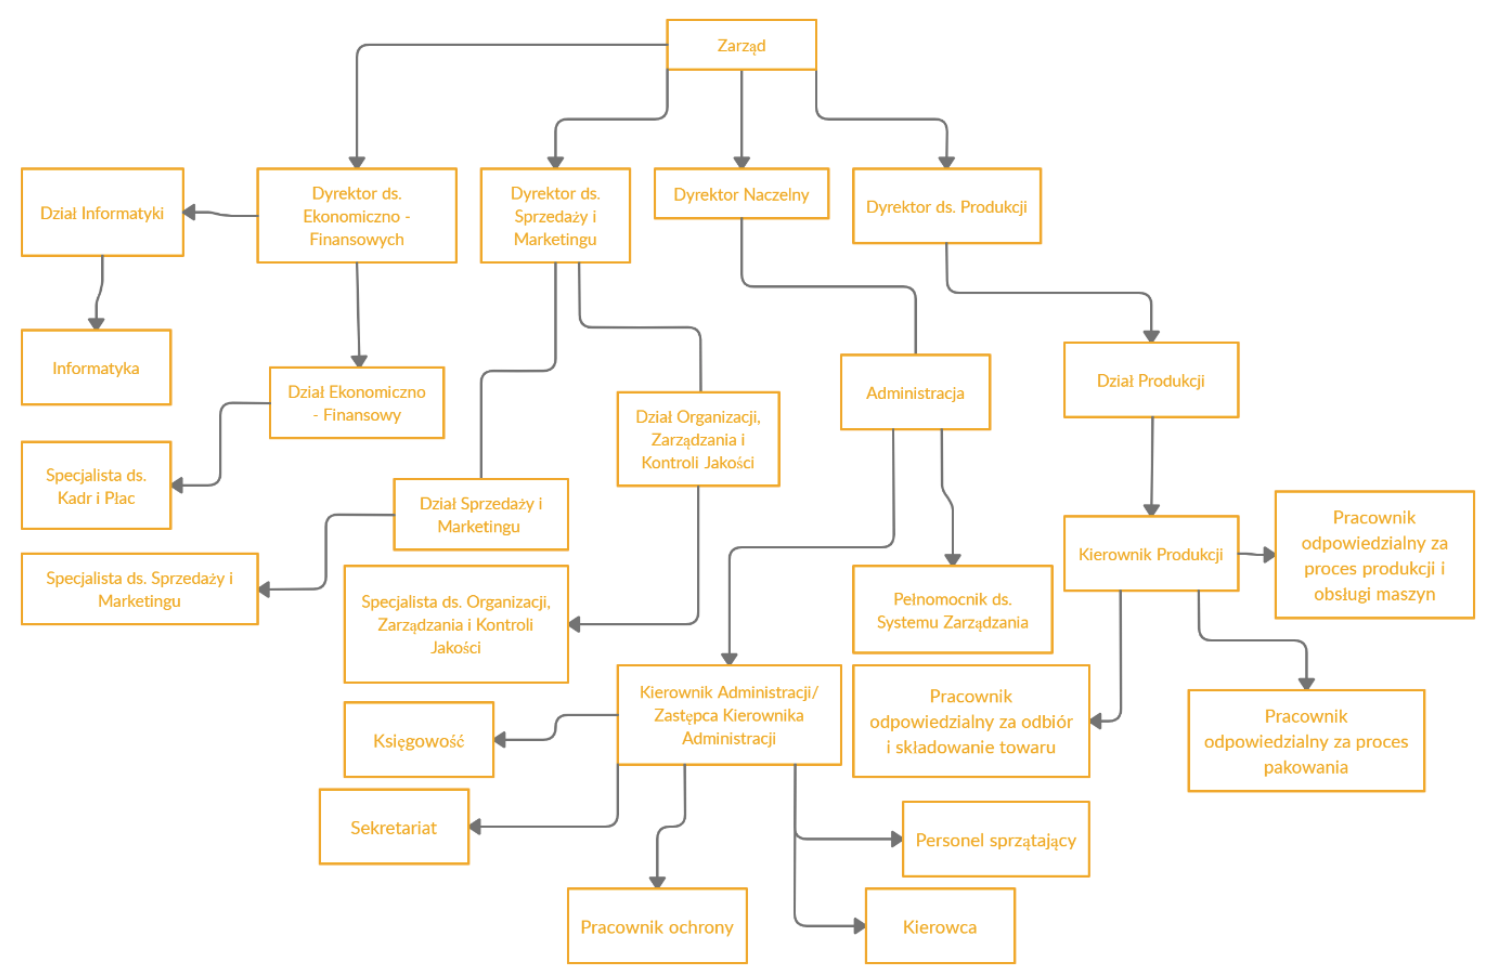
\includegraphics[width=0.8\textwidth]{./sec17/struktura_organizacyjna.png}
	\caption{Schemat struktury organizacyjnej (autor: Grzegorz Jakubiak)}
\end{figure}

		Została wybrana taka liczba pracowników, gdyż według kodeksu pracy musi być zachowana doba pracownicza, co oznacza, że wymagane jest 11h odpoczynku, a czas pracy nie może przekraczać 8h na dobę oraz 48h tygodniowo w przyjętym okresie rozliczeniowym. 


\section{Opis koncepcji zagospodarowania terenu}

\begin{figure}[h]
	\centering
	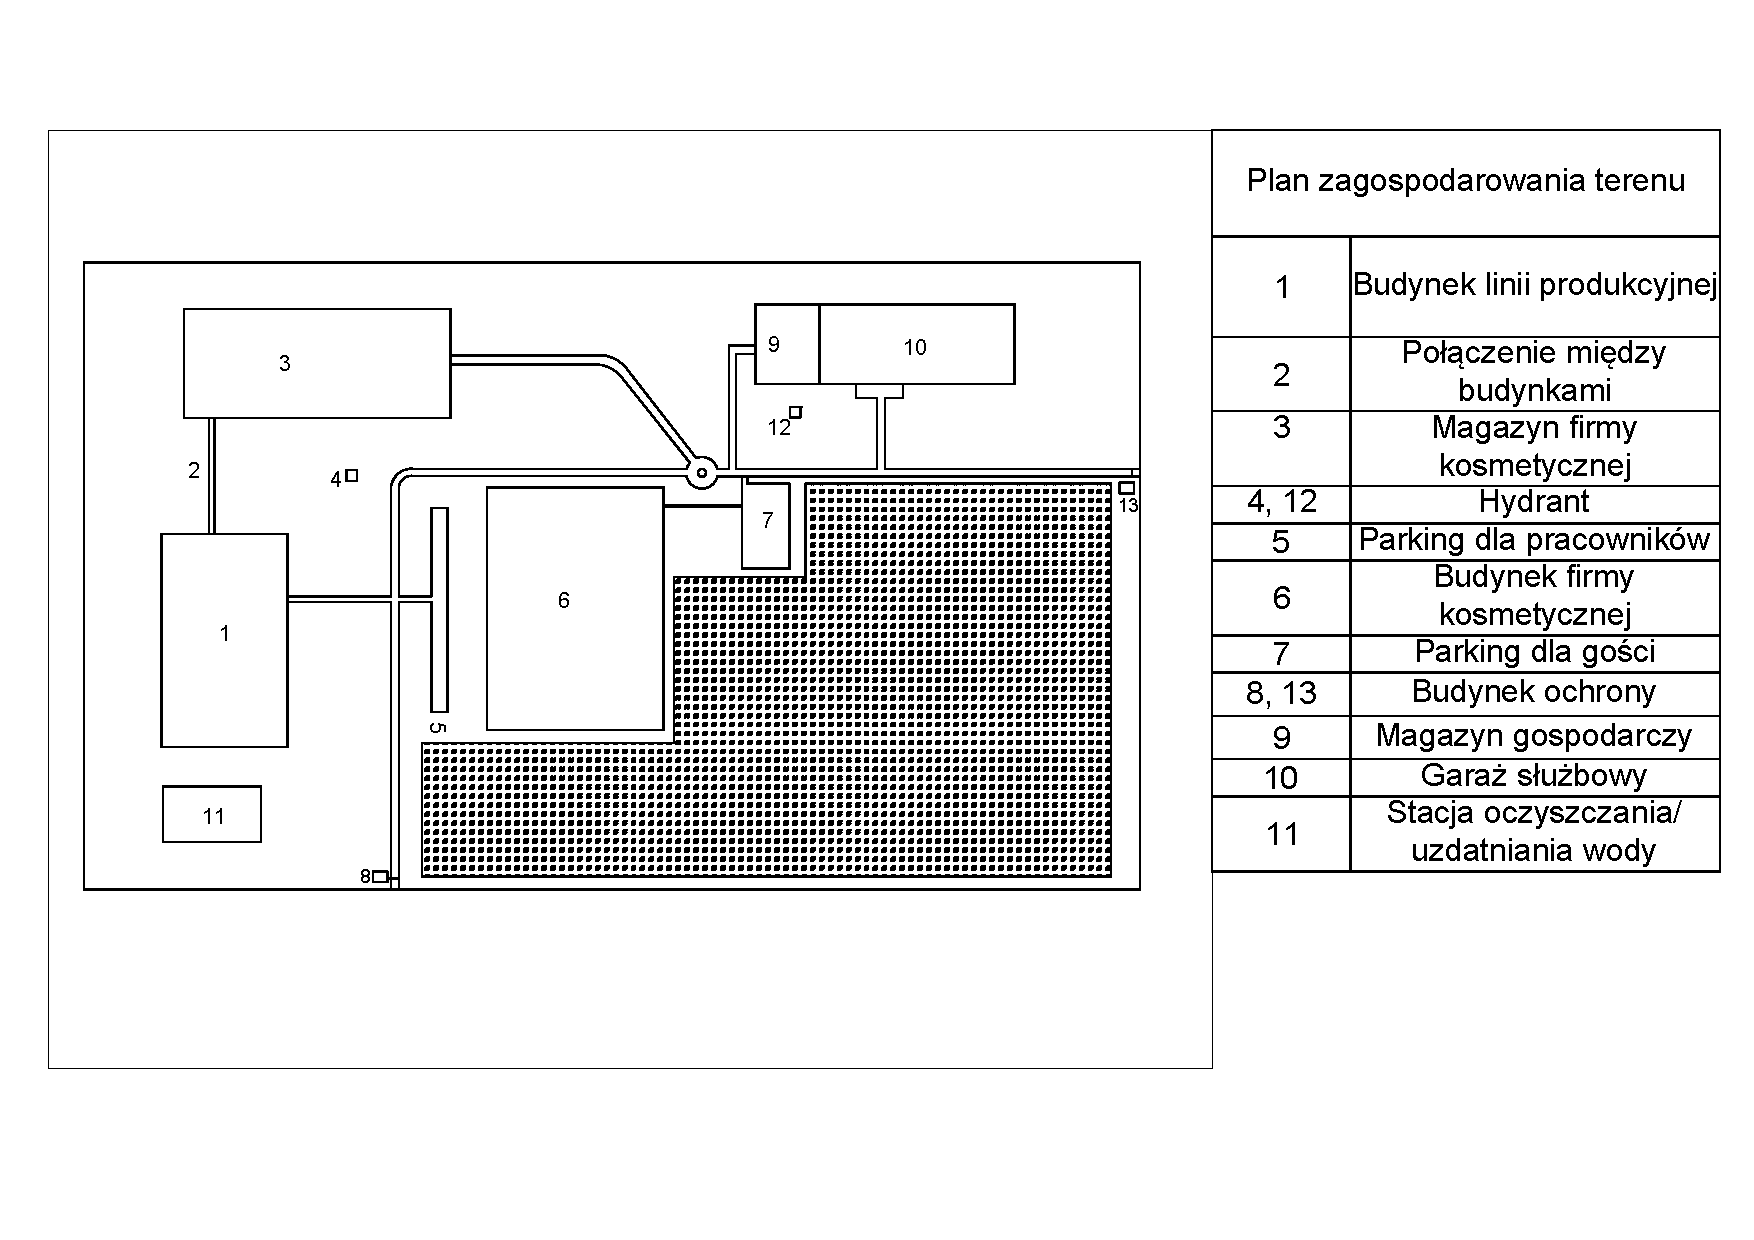
\includegraphics[width=0.95\textwidth]{./sec18/zagospodarowanie_terenu.pdf}
	\caption{Schemat planowanego zagospodarowania terenu (autor: Zuzanna Siek)}
\end{figure}


\section{Rodzaje odpadów i ich dobowa ilość}

Razem około 15tys. litrów ścieków na dobę. Odprowadzane do systemu kanalizacji.
\begin{itemize}
\item Ścieki technologiczne – woda zużyta do mycia aparatury i urządzeń oraz sprzątania pomieszczeń - około 3l na każdy litr produktu, czyli 14 tys. litrów na dobę
\item Ścieki bytowo-gospodarcze – produkowane przez pracowników - ok. 15l na jednego pracownika, czyli 1tys. litrów na dobę
\end{itemize}\vspace{\baselineskip}

Odpady są segregowane. Zakład ma podpisaną umowę z lokalną firmą zajmującą się wywozem i utylizacją śmieci. Odpady odbierane są z zakładu w każdy poniedziałek, środę oraz piątek.
\begin{itemize}
\item Opakowania po komponentach na kosmetyki – kartony, beczki, worki, palety
\item Wadliwe opakowania na kosmetyki
\item Odpady powstające na hali produkcyjnej
\item Odpady komunalne - związane z bytowaniem pracowników
\end{itemize}\vspace{\baselineskip}

Zakład ma podpisaną umowę z firmą zajmującą się utylizacją odpadów potencjalnie niebezpiecznych dla środowiska. Odpady odbierane są z zakładu w każdy poniedziałek.
\begin{itemize}
\item Próbki kosmetyków poddawane analizie w laboratorium
\item Odczynniki chemiczne używane do analiz oraz płytki z pożywkami i wyhodowanym na nich materiałem biologicznym
\item Opakowania po odczynnikach chemicznych
\item Wadliwe partie produktów
\end{itemize}


\section{Proponowane rozwiązania z zakresu ochrony środowiska}

\section{Kontrola jakości, rozpoznanie możliwości wdrożenia wybranych norm jakościowych}

Do głównych zadań kontroli jakości należy:
\begin{itemize}
	\item pobieranie prób
	\item przeprowadzanie badań -- materiałów wyjściowych oraz produktów gotowych
	\item badania stabilności produktów
	\item walidacja metod badawczych
\end{itemize}\vspace{\baselineskip}

W strukturze organizacyjnej wytwórni dział jakości zajmuje szczególne miejsce tzn. jest niezależny od każdej innej jednostki organizacyjnego. Posiada laboratorium z pracownikami i wyposażeniem umożliwiającym przeprowadzenie wszystkich niezbędnych kontroli i badań. Wszystkie dane i wyniki uzyskiwane podczas kontroli jakości muszą być wiarygodne, powtarzalne i oparte na solidnej wiedzy naukowej.\vspace{\baselineskip}

Laboratorium posiada procedury, instrukcje oraz określone specyfikacje dla wszystkich materiałów (produktów) oraz metody kontroli, aby mieć pewność, że:
\begin{itemize}
	\item osoby uprawnione posiadają wszystkie informacje konieczne, aby zdecydować czy dana seria produktu nadaje się do zwolnienia do obrotu
	\item drogą audytu możliwe jest odtworzenie historii każdej wytworzonej serii
\end{itemize}\vspace{\baselineskip}

W opracowanych dokumentach prowadzi się kontrolę wprowadzanych zmian, które są udokumentowane i uzasadnione. Archiwizowane są oryginału dokumentów, a stosowane nadzorowane kopie. Czas i miejsce przechowywania archiwalnych oryginałów jest określone; miejsce przechowywania odpowiednio zabezpieczone, aby zapewnić odpowiedni stan i czytelność archiwizowanych dokumentów.

Sprzęt wykorzystywany w laboratoriach kontroli jakości jest kalibrowany i sprawdzany odpowiednimi metodami, w określonych odstępach czasu; urządzenia niesprawne, w miarę możliwości usunięte lub wyraźne oznakowane jako nieprawne. Jeżeli wyposażenie nie podlega wzorcowaniu jest wyraźnie oznakowane w sposób odróżniające je od tego, które wymaga wzorcowania. Oznakowanie powinno pozwolić na stwierdzenie, kiedy ma być przeprowadzone następne wzorcowanie.

Ocena każdej i szczególnej serii produktu jest oparta na badaniach, które zostały przeprowadzone na reprezentacyjnej próbce. Próbka jest reprezentatywna, jeżeli dostarcza informacji całej serii materiału lub produktu.\vspace{\baselineskip}

Jeżeli próbka ma myc reprezentatywna to powinna zostać pobrana:
\begin{itemize}
	\item z materiału, który jest jednorodny
	\item w odpowiedni sposób
	\item za pomocą odpowiedniego sprzętu
	\item do odpowiednich pojemników
	\item w odpowiedniej tłuści
	\item w odpowiednim pomieszczeniu
	\item przez upoważnionego pracownika
	\item z zachowaniem należytych środków ostrożności i zasad BHP
\end{itemize}\vspace{\baselineskip}

Pobrane próbki do bieżących badań analitycznych i mikrobiologicznych oraz próbki archiwalne:
\begin{itemize}
	\item wyrobów gotowych, w opakowaniach bezpośrednich, w ilościach wystarczających na wykonanie 1-2 pełnych analiz zgodnych ze specyfikacją
	\item materiałów wyjściowych
\end{itemize}\vspace{\baselineskip}

Na podstawie wyników badań reprezentatywnej próbki upoważniona osoba podejmuje decyzje o zwolnieniu danej partii materiału do produkcji wyrobu gotowego do obrotu. Przy czym istotne są dwie zasady:
\begin{enumerate}
	\item Można używać tylko materiałów wyjściowych i opakowaniowych zwolnionych przez Dział Kontroli Jakości oraz będących w okresie ważności
	\item Żadna seria produktu nie może zostać zwolniona do obrotu zanim osoba uprawniona nie wyrazi pisemnej zgody potwierdzającej zgodność serii z wymaganiami określonymi w specyfikacji.
\end{enumerate}\vspace{\baselineskip}

Wszystkie podejrzane wyniki, które są niezgodne z wymaganiami specyfikacji lub ustalonymi kryteriami akaparacji określa się jako wyniki poza specyfikacją (OOS) i muszą być one wyjaśnione w toku specjalnego postępowania Działu Kontroli Jakości. Wynik OOS nie zawsze oznacza wadliwą serię i konieczność jej odrzucenia. Ważne jest jednak, aby każdy wynik OOS został zaszeregowany do jednego z 3 możliwych kategorii błędów:
\begin{itemize}
	\item błędu laboratoryjnego
	\item błędu produkcyjnego niezależnego od procesu
	\item błędu procesu produkcyjnego
\end{itemize}\vspace{\baselineskip}

Przebieg działań wyjaśniających wynik OOS musi być udokumentowany i szczegółowo opisany w specjalnym raporcie.


\section{Wskaźniki techniczno-ekonomiczne}

\newpage
\renewcommand*{\bibfont}{\small}
\printbibliography

\end{document}
